\documentclass[review,authoryear,3p,times]{elsarticle}
% EJOR submission -- v4 draft (2026-09-21): v3 rewritten shorter, plainer style.
%
% v3 REFRAME. v2 (main.tex, retained UNMODIFIED -- it is untracked, do not
% overwrite) was built around two mechanisms: s-ccf (component-factored credit)
% and cfpk (forked simulator replay). v3 is built around ONE mechanism,
% cgae-cflow: run GAE along the token-provenance DAG instead of the trajectory
% index. It needs no forking, no hand-specified factorization, and ~1 ms/episode.
%
% WHAT CARRIES OVER FROM v2 NEAR-VERBATIM: Section 2 (related work, plus two new
% paragraphs), Section 3 (background, plus a GAE subsection), and Section 7 (the
% boundary-condition investigation, unchanged). Those are marked \portold.
%
% CLAIM DISCIPLINE (see ../EJOR_PAPER_OUTLINE_V3.md 6.0 and 6a-40): all ncopies
% and s1 numbers here are at the CONVERGED 40-epoch budget. The 15-epoch
% protocol produced a significant but spurious result and must not be reported
% as primary. In particular v2's "beats ccf" framing is RETIRED: at converged
% budgets cgae-cflow does not beat ccf, cgae, or cgae-cap.

\usepackage{amsmath,amssymb,amsthm}
\usepackage{graphicx}
\usepackage{booktabs}
\usepackage{algorithm}
\usepackage{algpseudocode}
\usepackage{xcolor}
\usepackage{tikz}
\usetikzlibrary{petri,positioning,arrows.meta,fit,backgrounds,calc}
\usepackage[hidelinks]{hyperref}

% --- float placement: the defaults strand large floats at the end ------
\setcounter{topnumber}{3}
\setcounter{bottomnumber}{2}
\setcounter{totalnumber}{4}
\renewcommand{\topfraction}{0.9}
\renewcommand{\bottomfraction}{0.7}
\renewcommand{\textfraction}{0.08}
\renewcommand{\floatpagefraction}{0.75}

\newtheorem{proposition}{Proposition}
\newtheorem{corollary}{Corollary}
\newtheorem{assumption}{Assumption}
\newtheorem{remark}{Remark}
\newtheorem{lemma}{Lemma}
\newtheorem{definition}{Definition}

% --- estimator names -------------------------------------------------------
\newcommand{\cgae}{\textsc{cgae}}              % mean over successors
\newcommand{\cflow}{\textsc{cgae-cf}}          % THE METHOD: convex flow weights
\newcommand{\cflowraw}{\textsc{cgae-f}}        % predecessor-normalized (broken)
\newcommand{\cdag}{\textsc{cgae-dag}}          % exact closure semantics
\newcommand{\ccap}{\textsc{cgae-cap}}          % sub-stochastic ablation
\newcommand{\ccf}{\textsc{ccf}}
\newcommand{\sccf}{\textsc{s-ccf}}
\newcommand{\mcq}{\textsc{mc-q}}
\newcommand{\lrq}{\textsc{lrq}}
\newcommand{\cfgae}{\textsc{cfgae}}
\newcommand{\cfpk}{\textsc{cfpk}}

\newcommand{\Fscr}{\mathcal{F}}
\newcommand{\Ascr}{\mathcal{A}}
\newcommand{\Ex}{\mathbb{E}}
\newcommand{\Var}{\operatorname{Var}}
\newcommand{\Cov}{\operatorname{Cov}}
\newcommand{\desc}{\operatorname{desc}}
\newcommand{\anc}{\operatorname{anc}}
\newcommand{\pred}{\operatorname{pred}}
\newcommand{\suc}{\operatorname{succ}}
\newcommand{\own}{\operatorname{own}}

% --- drafting aids: make every gap LOUD -----------------------------------
% \gap{...}      a missing number or result, with what is needed
% \gapdisc{...}  a discussion paragraph that cannot be written until a gap fills
% \portold{}  content to be copied across from main.tex (v2)
\newcommand{\gap}[1]{{\color{red}\textbf{[GAP: #1]}}}
\newcommand{\gapdisc}[1]{%
  \par\medskip\noindent{\color{red}\textbf{[DISCUSSION PENDING]} #1}\par\medskip}
\newcommand{\portold}[1]{%
  \par\medskip\noindent{\color{blue}\textbf{[PORT FROM v2 main.tex: #1]}}\par\medskip}

\journal{European Journal of Operational Research}

\begin{document}

\begin{frontmatter}

\title{Causal-Order Advantage Estimation: Provenance-Aware Credit
Assignment for Reinforcement Learning in Dynamic Task Assignment}

\author[tue]{R. Lo Bianco}
\address[tue]{Eindhoven University of Technology, The Netherlands}

\begin{abstract}
Dynamic task assignment consists of routing arriving work to a limited number
of resources. When such a problem is modelled as an Action-Evolution Petri Net
(A-E PN) and solved with deep reinforcement learning, the simulator records the
\emph{provenance} of every token, that is, which earlier decisions each reward
descends from, and existing learning algorithms do not use this record. This
paper proposes to use it for credit assignment. Generalized Advantage
Estimation accumulates temporal-difference errors along the trajectory index,
but in a system running many concurrent cases the next decision usually
belongs to a different case, so its error carries little information about the
current action. We run the same recursion along the provenance graph instead.
The resulting estimator enters each reward once, at the latest decision on
its provenance, lets earlier decisions receive it through the recursion, and
combines provenance successors by a flow-weighted average normalized over
successors;
we show that the alternative normalization, over predecessors, leaves the
bootstrap coefficient unbounded and produces an error that grows with the
critic. Under a component mean-exogeneity assumption, whose scope we discuss,
scoping credit to a decision's provenance descendants leaves the expected
policy gradient unchanged and reduces its variance by a factor governed by the
number of reward-bearing causal components, $K$. On six problem configurations
spanning $K=1$ to $K=8$, the method improves normalized return over
discount-matched PPO by $+0.19$ to $+0.55$ (paired, $20$ seeds, $p\le0.002$) at
the four largest $K$ and is indistinguishable from it at the two smallest, at a
cost of about one millisecond per episode. Because $K$ is computable from
untrained rollouts, it indicates in advance where the method can be expected
to help. All experiments are conducted within the A-E PN ecosystem.
\end{abstract}

\begin{keyword}
reinforcement learning \sep credit assignment \sep dynamic task assignment \sep
Petri nets \sep decomposition \sep policy gradient
\end{keyword}

\end{frontmatter}

%===========================================================================
\section{Introduction}

Dynamic task assignment is the problem of deciding, repeatedly and under
uncertainty, which resource should serve which unit of work. It covers machine
scheduling, service operations, patient flow, order picking and vehicle
dispatching. What makes the modern instances hard is the combination of
stochastic arrivals, contended and heterogeneous resources, and an action space
whose size changes with the state. Recent work models such problems as
Action-Evolution Petri Nets (A-E PN) and solves them with deep reinforcement
learning (RL), which accommodates exactly that kind of action space
\citep{aepn2023,aepn_repr2025,gympn2025}.

In that line of work the model and the learner are developed separately. The
net is compiled into a semi-Markov decision process and handed to Proximal
Policy Optimization (PPO) with Generalized Advantage Estimation (GAE), and the
learning algorithm sees only states, actions and rewards. The execution trace
that the simulator produces while generating those quantities is not used as a
source of learning signal. This paper asks what is gained by using it.

The difficulty we address is credit assignment in concurrent systems. GAE
accumulates temporal-difference errors along the trajectory index,
$A_t = \delta_t + \gamma\lambda A_{t+1}$. In an A-E PN running many cases at
once, decision $t+1$ typically belongs to a different case from decision $t$,
so its reward is generated by tokens that the action at $t$ never touched.
Credit therefore propagates along wall-clock order, while the dependence
between decisions and rewards runs along the flow of tokens. This mismatch is
a consequence of concurrency, not of the state encoding, and the variance it
contributes grows with the number of cases in flight.

The simulator already records what is needed to remove the mismatch. For every
transition firing, an A-E PN simulation logs which tokens were consumed, which
were produced, when the firing occurred and what reward it emitted. Chaining
these records by token identity yields the \emph{provenance} of every reward:
the set of earlier decisions from whose outputs the reward's consumed tokens
descend. Provenance is a by-product of executing the net; it is not estimated
from data and it is not, by itself, a causal effect. It gives an exact
\emph{ancestry} relation, a necessary condition for one decision to have
influenced one reward, and we use it to decide which rewards a decision's
advantage is allowed to see. We keep this distinction explicit throughout
(Section~\ref{sec:terms}).

We leave the policy-gradient algorithm, the network and the objective
untouched and change one thing: the successor relation along which the
advantage recursion runs. Instead of accumulating from decision $t$ to decision
$t+1$ in firing order, we accumulate from a decision to its \emph{provenance
successors}, the decisions that consume tokens descending from it. Each reward
enters the recursion once, at a single owner, the latest decision on its
provenance; earlier decisions on that provenance receive it through the
recursion, as in GAE. Ownership therefore partitions the episode's reward and
the estimator is a return decomposition. Successors are combined by a weighted
average of their token-flow shares. The construction is purely structural: it needs no
token-value semantics, no hand-specified factorization and no re-run
simulation. We call it causal-order advantage estimation, where \emph{causal
order} refers to the provenance ancestry just described.

The contributions of this paper are the following.
\begin{enumerate}
\item A provenance-aware advantage estimator, \cflow{}
(Section~\ref{sec:method}): GAE with the temporal successor replaced by the
provenance successor, single-owner reward attribution and a convex
flow-weighted combination over successors. The credit factorization is derived
from the simulator's record, per episode, at a cost of about one millisecond.
\item The conditions under which the construction is justified, and a bias
analysis (Section~\ref{sec:theory}). We state a component mean-exogeneity
assumption, discuss when operational systems satisfy it, isolate a structural
condition on reward firings that is checkable on the trace, prove that under
both the closure estimand is unbiased for the policy gradient, and bound the
departure of the shipped estimator from that estimand by a quantity computable
before training.
\item The identification and repair of a normalization defect. The natural
flow-weighted form normalizes over the predecessors of each node, which is what
token conservation yields; but the recursion sums over successors, so the
coefficient multiplying the bootstrap is a row sum that the constraint does not
bound, and the resulting error is proportional to the critic. Normalizing over
successors removes it identically.
\item A pre-training diagnostic. The number of reward-bearing causal
components $K$ and the mean causal fan-out are computable from a few rollouts
of an untrained policy. Together they indicate where the method can help
($K>1$) and whether the successor-combination rule matters at all (fan-out
$>1$).
\item An empirical study within the A-E PN ecosystem (Section~\ref{sec:exp}):
a comparison against discount-matched PPO and seven alternative credit rules on
six problem configurations, an ablation ladder over the estimator family, and a
negative control on which the mechanism predicts and obtains a null.
\end{enumerate}

The findings are conditioned as follows. Causal-order estimation improves on
discount-matched PPO at the four configurations with the largest $K$, by
$+0.19$ to $+0.55$ in normalized return over $20$ paired seeds, and is
indistinguishable from it at the two with the smallest. Against other bounded
credit rules that scope credit by component it is statistically
indistinguishable, and we do not claim superiority over them. The
predecessor-normalized variant loses its learned policy late in training, and
the variant computing the causal estimand exactly is not the best member of the
family. On the one benchmark with headroom below the anchor, those two variants
and a third never learn at all (Section~\ref{sec:hard}). Every statement about
the expected policy gradient is conditional on Assumption~\ref{as:exo}, which
is plausible for systems that decompose into weakly coupled sub-streams and not
for systems in which one congested resource pool links all work
(Section~\ref{sec:a1scope}). All experiments are run within the A-E PN
ecosystem, so replication elsewhere remains to be done.

The remainder of this paper is structured as follows. Section~\ref{sec:related}
reviews related work. Section~\ref{sec:background} introduces A-E PN, the
induced decision process and the provenance record. Section~\ref{sec:method}
defines the estimator and Section~\ref{sec:theory} analyses it.
Section~\ref{sec:exp} reports the experiments, Section~\ref{sec:discussion}
discusses their interpretation, scope and limitations, and
Section~\ref{sec:conclusion} concludes.

%===========================================================================
\section{Related work}
\label{sec:related}

\paragraph{Deep RL for dynamic task assignment.} A growing literature applies
deep RL to scheduling, routing and business-process decision-making, typically
encoding the instance as a graph consumed by a graph neural network: greedy
graph-embedding heuristics \citep{khalil2017learning}, attention-based routing
\citep{nazari2018vrp} and graph-network dispatching for job-shop scheduling
\citep{zhang2020jobshop}; \citet{mazyavkina2021survey} and
\citet{bengio2021tour} survey the area. Within the A-E PN program,
\citet{aepn2023} introduce the formalism, \citet{aepn_repr2025} a graph
representation for infinite state and action spaces, and \citet{gympn2025} a
library supporting partial observability and multiple decisions. In all of this
work the effort goes into the encoding and the policy architecture, and the
simulator's execution trace is not used as a learning signal. Our contribution
is a credit-assignment mechanism, so it is compatible with and inherits from
that literature.

\paragraph{Credit assignment in RL.} Return decomposition \citep{rudder2019}
redistributes return along a trajectory with a learned return model, and
Hindsight Credit Assignment \citep{hca2019} reweights past actions by their
learned likelihood of having caused an outcome. Both are learned
redistributions. Token provenance is recorded exactly by the simulator, so the
step that decides which rewards a decision may be credited with introduces no
estimation error, although what is exact is the ancestry relation and not a
causal effect (Section~\ref{sec:terms}). Model-free counterfactual credit
assignment \citep{ccadeep2021} shares the motivation and builds low-variance
baselines by conditioning on future events; simulator-replay counterfactual
credit (\cfpk{}) is the exact, model-based end of the same spectrum, at a
simulation cost that \cflow{} avoids.

\paragraph{Factored and multi-agent credit.} Difference rewards
\citep{difference2002}, COMA \citep{coma2018} and value decomposition
\citep{vdn2018,qmix2018} credit each agent against a counterfactual baseline
or factor a joint value, and all require the entity partition to be supplied.
MACCA \citep{macca2024} learns the causal structure from offline data instead.
The distinction we draw is therefore \emph{learned versus recorded}: a
structure estimated from transition tuples carries estimation error, whereas an
A-E PN writes down, for each firing, which tokens were consumed and produced.
Our partition also changes per episode with the realized case mix, and it
factors a single-agent problem with many concurrent cases in the same way it
would a multi-agent one.

\paragraph{The simulator as more than a source of samples.}
\citet{diffdes2024} make the simulator differentiable and take pathwise policy
gradients through it; that needs smooth surrogate dynamics, where ours needs
only recorded token identity, and the two are complementary.
\citet{eventdriven2026} control a semiconductor fab and start from an
observation we share: because an action initiates an extended event that
overlaps others, the next decision point may be uninformative for credit
assignment. Their response groups events that co-occur in a time window and
matches the group to one system-level reward; ours groups the decisions from
whose outputs a reward's tokens descend and needs only the rewards the episode
already pays.

\paragraph{Decomposition in operations research.} Dantzig--Wolfe
\citep{dantzig1960decomposition} and Benders \citep{benders1962partitioning}
decomposition split a structured problem along a block structure identified by
hand. \cflow{} applies the same idea to the policy-gradient return, along a
block structure derived per episode from the simulator's record.

\paragraph{Generalized advantage estimation and deliberate bias.} Our estimator
is GAE \citep{gae2016} with one substitution, so GAE is the closest technical
antecedent. GAE with $\lambda<1$ is itself biased, and the biased settings are
the ones used in practice; its bias is a shrinkage by temporal distance,
$\lambda^k$, where ours shrinks by causal distance. We therefore relocate a
shrinkage that is already present rather than introduce one. Deliberate bias
is common in this pipeline (PPO's clipped surrogate, truncated importance
weights, reward clipping), and in our experiments the unbiased member of the
estimator family does not perform better than the biased one we ship.

\paragraph{Reward shaping and graph architectures.} Potential-based shaping
\citep{ng1999shaping} cannot change the optimal policy; we use its
SMDP-discounted form as one of three alternative routes tested in
\ref{app:boundary}. The policy is a Heterogeneous Graph Transformer
\citep{hu2020hgt}, the standard choice for encoding combinatorial structures of
variable size. That appendix also documents an architectural finding of
independent interest: a per-node actor decoder over directed-only
message-passing edges can be exactly blind to state outside its
forward-reachable neighbourhood, a limitation the pooling critic does not share.

%===========================================================================
\section{Background}
\label{sec:background}

This section describes the A-E PN formalism informally, defines the learning
problem, and fixes the terminology used in the rest of the paper.

\subsection{Action-Evolution Petri Nets and the induced decision process}

A Petri net is a bipartite directed graph of \emph{places} and
\emph{transitions}. Places hold \emph{tokens}; in a colored net each token
carries data, such as a task's type or a resource's identity. A transition is
\emph{enabled} when its input places hold a matching combination of tokens,
called a \emph{binding}, and \emph{firing} it consumes that binding and
produces tokens in its output places. The distribution of tokens over places,
the \emph{marking}, is the system state.

An A-E PN \citep{aepn2023} partitions the transitions into two kinds and adds a
global clock. \emph{Evolution} transitions model the exogenous dynamics, such
as arrivals and service completions; they fire automatically according to
stochastic timed rules and advance the clock. \emph{Action} transitions model
the controllable decisions: whenever several action bindings are enabled at
once, a \emph{policy} selects which one to fire. Any firing may emit a scalar
reward. Figure~\ref{fig:aepn} shows a minimal assignment net.

\begin{figure}[tbp]
\centering
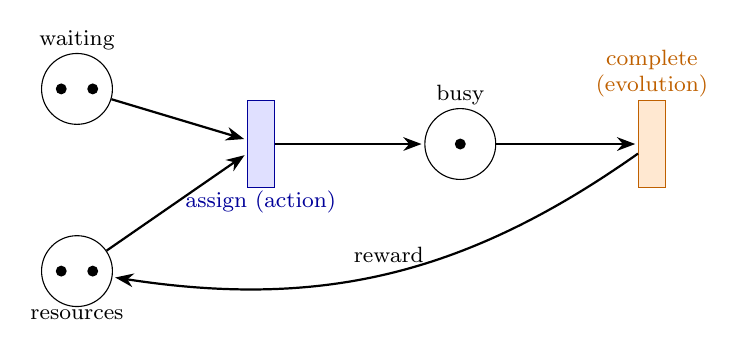
\begin{tikzpicture}[>=Stealth,node distance=1.5cm,
  place/.style={circle,draw,minimum size=9mm,inner sep=1pt},
  tok/.style={circle,fill=black,inner sep=1.4pt},
  act/.style={rectangle,draw=blue!60!black,fill=blue!12,minimum width=3.4mm,minimum height=11mm},
  evo/.style={rectangle,draw=orange!75!black,fill=orange!18,minimum width=3.4mm,minimum height=11mm},
  arc/.style={->,thick,shorten >=1pt},
  every label/.style={font=\footnotesize,inner sep=1pt,align=center}]
  \node[place,label=above:{\footnotesize waiting}] (w) {};
    \node[tok] at ([xshift=-2mm]w.center){}; \node[tok] at ([xshift=2mm]w.center){};
  \node[place,below=1.4cm of w,label=below:{\footnotesize resources}] (r) {};
    \node[tok] at ([xshift=-2mm]r.center){}; \node[tok] at ([xshift=2mm]r.center){};
  \node[act,right=1.7cm of w,yshift=-0.7cm,label=below:{\footnotesize\color{blue!60!black}assign (action)}] (a) {};
  \node[place,right=1.9cm of a,label=above:{\footnotesize busy}] (b) {};
    \node[tok] at (b.center){};
  \node[evo,right=1.8cm of b,yshift=0cm,
        label={[text=orange!75!black]above:{\footnotesize complete\\(evolution)}}] (c) {};
  \draw[arc] (w) -- (a);
  \draw[arc] (r) -- (a);
  \draw[arc] (a) -- (b);
  \draw[arc] (b) -- (c);
  \draw[arc] (c) to[bend left=22] node[above,font=\footnotesize] {reward} (r);
\end{tikzpicture}
\caption{A minimal A-E PN for task assignment. The \emph{assign} action
transition (blue) is a decision point; the \emph{complete} evolution transition
(orange) fires after a stochastic delay, returns the resource and emits a
reward.}
\label{fig:aepn}
\end{figure}

Execution alternates between the environment evolving the marking and the
agent choosing among enabled action bindings, which is a semi-Markov decision
process (SMDP). We write $s_d$ for the marking at decision $d$, $a_d$ for the
chosen binding and $u_d$ for its clock. Delayed rewards are discounted by the
SMDP factor $\rho_d(t)=e^{-\beta\max(0,\,t-u_d)}$. The policy $\pi_\theta$ is a
graph neural network over the assignment-graph representation of
\citet{aepn_repr2025}, trained by PPO \citep{ppo2017} with GAE
\citep{gae2016}. GAE forms $A_t=\sum_{k\ge0}(\gamma\lambda)^k\delta_{t+k}$ with
$\delta_t=r_t+\gamma V(s_{t+1})-V(s_t)$, computed by the backward recursion
$A_t=\delta_t+\gamma\lambda A_{t+1}$. Everything below changes only the
successor $t+1$ in this recursion.

Executing an A-E PN produces, for each firing, a record of the input tokens
consumed, the output tokens produced, the firing time and the reward emitted.
Writing $\Ascr$ for the set of agent decisions in an episode, indexed in firing
order, the record induces a directed acyclic graph on $\Ascr$: token identity
links each consumed token back to the firing that produced it, transitively
through evolution and forced firings. We call this the provenance DAG.

\subsection{Provenance, causal ancestry and causal effect}
\label{sec:terms}

Three notions must be kept apart. \emph{Token provenance} is the recorded
relation: composing the firing records by token identity gives, for any token,
the firings from whose outputs it descends. It is exact and observational, a
property of the executed trajectory. \emph{Causal ancestry} is the relation we
derive from it: decision $d$ is a causal ancestor of reward $r_j$ if some token
consumed at $j$'s firing descends from an output token of $d$. Because a reward
in an A-E PN is a deterministic function of the tokens consumed at its firing,
ancestry is a necessary condition for $d$ to have influenced $r_j$, and not a
sufficient one: a decision may be an ancestor of a reward that would have been
earned in the same amount under any other action. \emph{Marginal causal
effect} is what a counterfactual quantity such as a difference reward measures,
and estimating it requires re-running the simulator or learning a model of the
counterfactual. We do neither.

The estimator of Section~\ref{sec:method} uses ancestry as a scoping device: it
decides which rewards enter a decision's advantage and leaves the magnitude of
credit to the ordinary policy-gradient machinery. Throughout, the word
``causal'' in \emph{causal successor}, \emph{causal component} and \emph{causal
depth} refers to this ancestry relation, never to an estimated effect size. The
one place where causality in the stronger sense enters is
Assumption~\ref{as:exo}, which is an assumption about the system and not
something the record can establish.

%===========================================================================
\section{Method: causal-order advantage estimation}
\label{sec:method}
%===========================================================================

% The lineage / causal-order mechanism figure. \input from main_v3.tex.
% Panel (a) is the paper's central idea in one picture: GAE bootstraps from the
% TEMPORAL successor, which in an interleaved system belongs to a different case;
% causal-order estimation bootstraps from the CAUSAL successor instead.
% Panel (b) is the normalization that Proposition 1 turns on.
\begin{figure}[t]
\centering
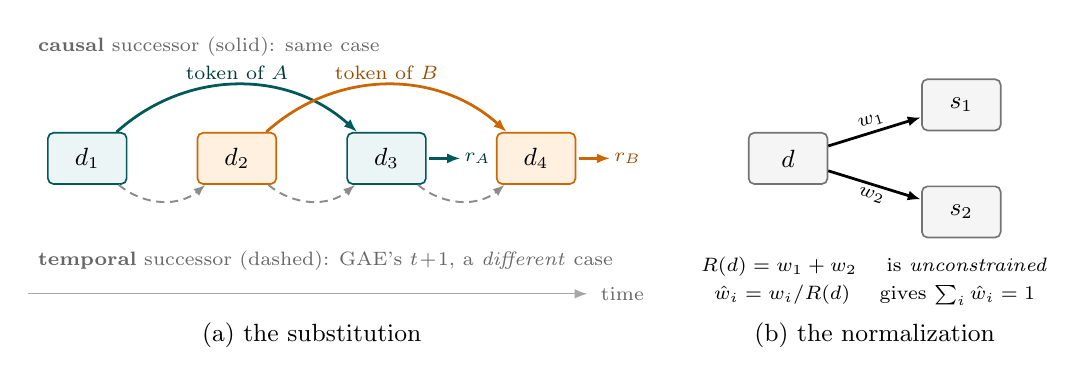
\begin{tikzpicture}[
  dec/.style={draw, rounded corners=2pt, minimum height=6.5mm,
              minimum width=10mm, align=center, font=\small, line width=0.6pt},
  caseA/.style={dec, fill=teal!8,   draw=teal!70!black},
  caseB/.style={dec, fill=orange!12, draw=orange!80!black},
  plain/.style={dec, fill=black!4,  draw=black!55},
  causalA/.style={-{Latex[length=1.7mm]}, line width=1.0pt, teal!70!black},
  causalB/.style={-{Latex[length=1.7mm]}, line width=1.0pt, orange!80!black},
  temporal/.style={-{Latex[length=1.5mm]}, densely dashed, line width=0.7pt,
                   black!45},
  tag/.style={font=\scriptsize, inner sep=1.5pt},
  note/.style={font=\scriptsize, black!60},
]

% ================= panel (a): temporal vs causal successor =================
\node[caseA] (d1) at (0,0)   {$d_1$};
\node[caseB] (d2) at (1.9,0) {$d_2$};
\node[caseA] (d3) at (3.8,0) {$d_3$};
\node[caseB] (d4) at (5.7,0) {$d_4$};

% causal recursion: solid arcs ABOVE, one per case
\draw[causalA] (d1) to[bend left=42]
  node[midway, above, tag, teal!45!black] {token of $A$} (d3);
\draw[causalB] (d2) to[bend left=42]
  node[midway, above, tag, orange!60!black] {token of $B$} (d4);

% temporal recursion: dashed arcs BELOW, consecutive, with visible heads
\foreach \a/\b in {d1/d2, d2/d3, d3/d4}
  \draw[temporal] (\a) to[bend right=40] (\b);

% rewards, emitted at the consuming decision
\draw[causalA] ($(d3.east)+(0.03,0)$) -- ++(0.40,0)
  node[right, tag, teal!45!black, inner sep=1pt] {$r_A$};
\draw[causalB] ($(d4.east)+(0.03,0)$) -- ++(0.40,0)
  node[right, tag, orange!60!black, inner sep=1pt] {$r_B$};

% legends for the two arrow families
\node[note, anchor=west, align=left] at (-0.75,1.42)
  {\textbf{causal} successor (solid): same case};
\node[note, anchor=west, align=left] at (-0.75,-1.30)
  {\textbf{temporal} successor (dashed): GAE's $t\!+\!1$, a \emph{different} case};

\draw[-{Latex[length=1.6mm]}, black!35] (-0.75,-1.72) -- (6.35,-1.72);
\node[note, anchor=west] at (6.4,-1.72) {time};

\node[font=\small] at (2.85,-2.25) {(a) the substitution};

% ================= panel (b): the successor normalization =================
\begin{scope}[xshift=8.9cm]
  \node[plain] (dd) at (0,0)      {$d$};
  \node[plain] (s1) at (2.2,0.68) {$s_1$};
  \node[plain] (s2) at (2.2,-0.68){$s_2$};

  \draw[-{Latex[length=1.7mm]}, line width=1.0pt] (dd) --
    node[midway, above, sloped, tag] {$w_1$} (s1);
  \draw[-{Latex[length=1.7mm]}, line width=1.0pt] (dd) --
    node[midway, below, sloped, tag] {$w_2$} (s2);

  % formulas: \textstyle keeps the sum limits inline, so nothing collides
  \node[anchor=north, align=center, font=\scriptsize, inner sep=2pt]
    at (1.1,-1.18)
    {$R(d)=w_1+w_2$ \quad is \emph{unconstrained}\\[2pt]
     $\hat w_i = w_i/R(d)$ \quad gives $\textstyle\sum_i \hat w_i = 1$};

  \node[font=\small] at (1.1,-2.25) {(b) the normalization};
\end{scope}

\end{tikzpicture}
\caption{The mechanism. \textbf{(a)} Four decisions in wall-clock order, drawn
from two interleaved cases $A$ and $B$. Generalized advantage estimation
bootstraps along the dashed \emph{temporal} chain, so the TD error it charges to
$d_1$ is the one produced at $d_2$---a decision about a different case, whose
reward $d_1$ did not influence. The token $d_1$ produced is instead consumed at
$d_3$, where the reward $r_A$ is emitted. Causal-order estimation follows the
solid provenance edges, so $d_1$ is credited with $r_A$ and never with $r_B$.
Reward ownership is a partition---each reward is assigned to the latest decision
on its own lineage---so no reward is counted twice. \textbf{(b)} Where a
decision's tokens feed several later decisions, the edge weights must be
normalized \emph{over successors}. Token conservation constrains the sum over
each node's predecessors, which leaves the row sum $R(d)$ free; because $R(d)$
multiplies the bootstrapped value (Proposition~\ref{prop:s}), leaving it
unbounded makes the recursion diverge in training.}
\label{fig:lineage}
\end{figure}


This section defines the estimator in three steps: the successor relation, the
ownership of rewards, and the recursion. Figure~\ref{fig:lineage} illustrates
the construction on a short episode.

\paragraph{Causal successors.} For a decision $d\in\Ascr$, $s\in\suc(d)$ when
$s$ consumes a token descending from an output token of $d$ with no
intervening decision. This is the \emph{nearest producer} relation: evolution
and forced firings are transparent, and the backward walk from a consumed token
stops at the most recent decision on its provenance. We call $\suc(d)$ the
causal successors of $d$. The relation is read off the execution record and
requires no token-value semantics.

Under token-flow postponement, a \textsc{postpone} decision re-emits the whole
marking and therefore stops the nearest-producer walk although it did not
originate the flow. Making postponements transparent recovers provenance edges
(measured at $97$ per episode on the single-component environment) and yields
a more faithful graph, but degrades learning (\ref{app:falsified}). We report
this as a measured boundary of the specification and keep postponements
opaque.

\paragraph{Single-owner reward attribution.} Let $\Ascr(j)$ be the set of
decisions in reward $j$'s ancestry. Each reward $r_j$ is assigned to the latest
decision on its lineage, $\own(j)=\arg\max_{d\in\Ascr(j)}u_d$. Ownership is a partition:
every reward is counted exactly once. This is what makes the estimator a return
decomposition rather than a hindsight $Q$-sample, in which every decision on a
lineage would receive the reward's full mass.

\paragraph{The recursion.} Let $w(d\!\to\!s)$ be the share of $s$'s consumed
tokens that descend from $d$, so that token conservation gives
\begin{equation}
\sum_{d\in\pred(s)} w(d\!\to\!s) = 1 .
\label{eq:predsum}
\end{equation}
Define the row sum and the successor-normalized weights
\begin{equation}
R(d) = \sum_{s\in\suc(d)} w(d\!\to\!s), \qquad
\hat{w}(d\!\to\!s) = \frac{w(d\!\to\!s)}{R(d)},\qquad
\sum_{s\in\suc(d)}\hat{w}(d\!\to\!s)=1 ,
\label{eq:sucsum}
\end{equation}
with $\hat w(d\!\to\!s)=1/|\suc(d)|$ when $R(d)=0$. With
$\rho(\Delta t)=e^{-\beta\Delta t}$ the SMDP discount applied at causal depth,
the estimator is
\begin{equation}
A[d] \;=\; \mathrm{owned}[d] - V[d]
\;+\; \sum_{s\in\suc(d)} \hat{w}(d\!\to\!s)\,\rho(u_s-u_d)\,
      \bigl( V[s] + \lambda A[s] \bigr),
\label{eq:cflow}
\end{equation}
evaluated by one backward pass over $\Ascr$ in decreasing clock order and
emitted as $Q[d]=A[d]+V[d]$. It is consumed like every other credit scheme: the
policy uses $A_d=Q[d]-V(s_d)$ and the value head regresses on $Q[d]$, so the
critic converges to the object the recursion bootstraps through.
Algorithm~\ref{alg:cflow} in \ref{app:defs} states the procedure line by line.

Three properties follow directly. Where every causal edge has out-degree one,
$\hat w\equiv1$ and \eqref{eq:cflow} reduces to ordinary SMDP-GAE, which we
verify to floating point on real traces. Under equal inflow shares
$\hat w=1/|\suc(d)|$, so the mean-over-successors rule (\cgae) is the
equal-share instance of \eqref{eq:cflow}. A \textsc{postpone} decision receives
the SMDP temporal-difference advantage $e^{-\beta\tau}V(s')-V(s)$, so that every
arm supports postponement in the same way. The computation costs about one
millisecond per episode, under $8\%$ of a training iteration.

%===========================================================================
\section{Theoretical analysis}
\label{sec:theory}
%===========================================================================

This section places \cflow{} in a family of estimators, identifies the member
that is unbiased for the policy gradient and the assumptions this needs, shows
why the bootstrap coefficient must be bounded, quantifies the variance
reduction, and bounds the bias of the estimator we ship relative to the
unbiased member. Proofs are in \ref{app:proofs}.

\subsection{A common form for the estimator family}

Every variant we consider is a choice of edge coefficient $c(d\!\to\!s)$ in
\eqref{eq:cflow}. Unrolling with $\lambda=1$ and $V\equiv0$,
\begin{equation}
Q[d] \;=\; \sum_{j\,:\,\own(j)\in\desc^{*}(d)} c_d(j)\,\rho(u_j-u_d)\,r_j,
\qquad
c_d(j)=\!\!\sum_{\text{paths } d\rightsquigarrow \own(j)}\ \prod c ,
\label{eq:unroll}
\end{equation}
so a variant is characterized by the total path weight it places on each
descendant's owned reward. Table~\ref{tab:family} lists the family.

\begin{table}[tbp]
\centering
\caption{The estimator family, and the two sums that matter.}
\label{tab:family}
\begin{tabular}{llcc}
\toprule
variant & $c(d\!\to\!s)$ & $\sum_{\pred(s)} c$ & $\sum_{\suc(d)} c$ \\
\midrule
\cdag  & $1$ (closure, set semantics)      & ---            & convex \\
\cflow & $w/R$                             & unbounded      & $=1$ exactly \\
\cgae  & $1/|\suc(d)|$                     & unbounded      & $=1$ exactly \\
\ccap  & $w/\max(R,1)$                     & $\le 1$        & $\le 1$ \\
\cflowraw & $w$                            & $=1$ exactly   & \textbf{unbounded} \\
\bottomrule
\end{tabular}
\end{table}

\subsection{The causal partition, the estimand and its unbiasedness}
\label{sec:estimand}

Write $\desc(d)$ for the set of decisions reachable from $d$ under the
successor relation, $\desc^{*}(d)=\desc(d)\cup\{d\}$, and
$\anc^{*}(e)=\{d:e\in\desc^{*}(d)\}$. Separately, build an undirected graph on
$\Ascr$ with an edge $(d,d')$ whenever some reward has both on its provenance;
its connected components are the \emph{causal components}, and $c(d)$ is the
component of $d$. Every reward with non-empty ancestry has a well-defined
component $c(j)$, and rewards with empty ancestry are constants that drop out
of the gradient. Note that $\desc^{*}(d)\subseteq c(d)$.

\begin{definition}[The structural statistic $K$]
\label{def:k}
$K$ is the number of causal components containing at least one reward,
computed per episode and averaged over rollouts of an untrained policy. It is a
real number rather than an integer, which is why the values $2.0$, $3.3$ and
$6.3$ reported for the $N$-copies benchmark sit at or below $N$. It requires no
training and no reward model.
\end{definition}

For decision $d$ let
\[
  G_d^{\mathrm{full}}=\sum_{j:\,t_j\ge u_d}\rho_d(t_j)\,r_j,
  \qquad
  \Delta_d=\sum_{\substack{j:\,t_j\ge u_d\\ c(j)\neq c(d)}}\rho_d(t_j)\,r_j ,
\]
so that $G_d^{\mathrm{full}}$ is the ordinary SMDP return-to-go used by PPO and
by the lineage ablation \mcq{}, and $\Delta_d$ is the part of it generated by
other components. Let $\Fscr_d$ be the history up to but excluding $a_d$. We
take the policy-gradient theorem in its causality form as given: the estimator
$\sum_d\nabla\log\pi(a_d\mid s_d)(G_d^{\mathrm{full}}-V(s_d))$ is unbiased for
$\nabla_\theta J$.

\begin{assumption}[Component mean-exogeneity]
\label{as:exo}
For every decision $d$,
$\;\Ex[\Delta_d \mid \Fscr_d,\,a_d] = \Ex[\Delta_d \mid \Fscr_d]$: given the
pre-action history, the expected cross-component future reward does not depend
on the action taken at $d$.
\end{assumption}

We refer to this assumption as (A1). A-E PN semantics supply part of the
argument for it. A reward is a deterministic function of the tokens consumed
at its firing, so along the realized execution $r_j$ can have been influenced
by $a_d$ only if $d\in\Ascr(j)$, hence only if $c(j)=c(d)$. But (A1) concerns
the conditional distribution over executions, including those that a different
action would have induced. Two channels can break it. The exogenous randomness
driving cross-component events must be, in conditional mean, unaffected by
$a_d$; this holds under independent per-firing draws, and Remark~\ref{rem:rng}
treats a single shared random stream. The substantive channel is
\emph{contention}: if the action at $d$ occupies or releases a resource that
work in another component would otherwise have used, that component's reward
stream shifts in distribution even though no token links the two. The record
cannot detect this, because the coupling acts through what did not happen.
Whether (A1) is tenable is therefore a question about the system, and
Section~\ref{sec:a1scope} discusses it.

\paragraph{The closure estimand.} The first row of Table~\ref{tab:family} is
the $c\equiv1$ member: the $\lambda=1$, $V\equiv0$ estimator crediting $d$ with
each descendant's owned reward exactly once,
\begin{equation}
  A^{\star}[d] \;=\; \sum_{j\,:\,\own(j)\in\desc^{*}(d)} \rho_d(t_j)\,r_j .
  \label{eq:star}
\end{equation}
\cdag{} computes it by construction, which we verify against the definition to
$0$ units in the last place over $191$ decisions. Because ownership is a
partition, each reward enters \eqref{eq:star} at most once even when its owner
is reachable from $d$ along several paths.

Unbiasedness needs two further conditions, which are verifiable on the trace.

\begin{assumption}[Time-forward causal edges]
\label{as:time}
$u_s > u_d$ for every causal edge $d\!\to\!s$.
\end{assumption}

\begin{assumption}[Single-origin rewards]
\label{as:origin}
For every reward $r_j$ with $\Ascr(j)\neq\emptyset$, the tokens consumed at
$j$'s firing have a single nearest-producer decision $a_j$.
\end{assumption}

Assumption~\ref{as:time} makes the provenance DAG acyclic and makes the
discount telescope along any path. Assumption~\ref{as:origin} holds whenever a
reward is earned by completing one unit of work whose most recent handling was
a single decision, which is the ordinary case in task assignment. It fails for
a \emph{join} reward, earned by a firing that consumes tokens last touched by
two different decisions. On all six configurations of this paper it holds on
every reward (Section~\ref{sec:exp}).

\begin{lemma}[Ownership dominates the ancestry]
\label{lem:own}
Under Assumptions~\ref{as:time} and \ref{as:origin},
$\own(j)=a_j$ and $\Ascr(j)\subseteq\anc^{*}(\own(j))$. Consequently, for every
decision $d$, $\own(j)\notin\desc^{*}(d)$ implies
$\Ascr(j)\cap\desc^{*}(d)=\emptyset$.
\end{lemma}

\begin{proposition}[The closure estimand is unbiased]
\label{prop:star}
Under Assumptions~\ref{as:exo}, \ref{as:time} and \ref{as:origin}, the estimator
$\hat g^{\star}=\sum_{d}\nabla_\theta\log\pi_\theta(a_d\mid s_d)\bigl(A^{\star}[d]-V(s_d)\bigr)$
satisfies $\Ex[\hat g^{\star}]=\nabla_\theta J(\theta)$ for any
$\Fscr_d$-measurable baseline $V$.
\end{proposition}

Proposition~\ref{prop:star} licenses \eqref{eq:star} as a reference point and
every relative statement made below. It says nothing about performance:
\cdag{} computes \eqref{eq:star} exactly and is one of the worst arms we
measured. The proof applies mean-exogeneity in a slightly broader form than
(A1) states, extending it to rewards in $d$'s own component whose owner lies
outside the descendant closure; Lemma~\ref{lem:own} places those rewards
outside $d$'s provenance descendants entirely, so the only channel by which
$a_d$ could move them is the contention channel that threatens (A1) itself.
Where Assumption~\ref{as:origin} fails, the broader form is genuinely stronger.

\subsection{The domain of validity of Assumption~\ref{as:exo}}
\label{sec:a1scope}

Call a system \emph{decomposable} at the scale of an episode when the work in
flight partitions into sub-streams drawing on disjoint capacity, so that an
assignment inside one sub-stream neither consumes nor delays capacity available
to another. Call it \emph{strongly coupled} when a single contended resource
serves all work, so that every assignment changes when that resource next
becomes free to everything else. (A1) is a natural modelling assumption at the
first extreme and is not credible at the second. Real systems lie between, and
their position is a design variable: the resource-pooling and flexibility
literature studies exactly this dial, since flexible capacity buys performance
by creating the cross-stream coupling that (A1) rules out
\citep{pooling_flexibility}.

The condition is approximately met wherever capacity is segmented and the
segments are not close to saturation: multi-site service operations with
site-dedicated staff, parallel production lines with their own operators,
regional fleets, wards with ring-fenced beds, picking zones with zone-assigned
pickers. It fails wherever sub-streams share capacity, and more generally under
congestion: a shared queue, a finite buffer that can block an upstream stage,
rework that returns work to a common queue, cross-trained staff who float
between sites. Even in the favourable cases, escalation paths and overflow
rules reintroduce coupling, and (A1) is stated per decision, so it can hold for
most decisions in an episode and fail for the few that touch a shared resource.
Our single-component environment (\ref{app:envs}) is a deliberate instance of
the coupled extreme.

$K$ (Definition~\ref{def:k}) measures how far an episode's realized provenance
decomposes. $K>1$ is necessary for (A1) to have content, but not sufficient,
because $K$ is computed from executions that did happen and cannot see the
contention channel. We therefore treat $K$ as a screening statistic and the
assessment of (A1) as a modelling judgement informed by it. Which results
depend on (A1) is stated precisely: Propositions~\ref{prop:star} and
\ref{prop:k} hold only under it, and so does every statement phrased relative
to the closure estimand. Propositions~\ref{prop:s} and \ref{prop:bias},
Lemma~\ref{lem:visit} and Proposition~\ref{prop:rel} are algebraic identities
about the recursion and hold regardless. If (A1) fails, \cflow{} remains a
bounded estimator whose departure from a well-defined reference is controlled,
but its expected gradient is no longer that of the objective. The one datum we
have on this case, the $K=1$ negative control, shows a null rather than a
degradation relative to PPO.

\subsection{Why the bootstrap coefficient must be bounded}

\begin{proposition}[Successor normalization]
\label{prop:s}
For the recursion \eqref{eq:cflow} with coefficient $c$, the coefficient
multiplying the bootstrap term at $d$ is $\sum_{s\in\suc(d)}c(d\!\to\!s)$. The
predecessor constraint \eqref{eq:predsum} does not bound this quantity. Writing
$\hat{G}(d)=\sum_s \hat w\,\rho\,(V[s]+\lambda A[s])$ for the estimator's own
bootstrapped continuation value, the unnormalized and normalized forms differ by
\begin{equation}
A_{\cflowraw}[d]-A_{\cflow}[d] \;=\; \bigl(R(d)-1\bigr)\,\hat{G}(d).
\label{eq:defect}
\end{equation}
\end{proposition}

The proof is immediate from $w=R\hat w$. On the single-component environment
$R(d)$ has mean $1.008$ and standard deviation $0.542$ over the range
$[0.143,3.429]$ (Figure~\ref{fig:rowsum} in \ref{app:cosine}), so a mean of
about $1$ conceals a dispersion problem. Three consequences follow. First, the
error scales with the critic, not the reward: $\hat{G}(d)=O(V)=O(H\bar r)$ for
remaining causal horizon $H$ and mean per-decision reward $\bar r$, while the
action-attributable signal is $\mathrm{owned}[d]=O(\bar r)$, so the estimator
degrades as the critic improves. Second, the error does not cancel as a
baseline: $R(d)$ depends on the realized DAG downstream of $d$, hence on the
action at $d$; forking every action at a decision state under common random
numbers, $R$ is identical across actions at only $18.8\%$ (four copies) and
$6.2\%$ (single component) of fork points. Third, successor normalization
removes the error identically, since $\sum_s\hat w=1$ gives $R\equiv1$.

\begin{remark}[The predecessor sum is a choice of estimand, not a defect]
\label{rem:p}
Reading \eqref{eq:predsum} as a second conservation requirement would admit
only $c=w/\max(R,1)$; the policy-gradient argument does not require it, since
nothing there constrains advantages across different decisions to sum to
anything. $\sum_{\pred(s)}c>1$ means each of $s$'s joint ancestors is credited
with the whole continuation, the but-for reading behind difference-reward
methods. Empirically the distinction barely moves total credit mass
($\sum_d Q[d]/G$ is $4.74$ for \cflowraw{} against $4.86$ for \cflow{} on the
single-component environment), and forcing the predecessor sum down (\ccap)
costs performance.
\end{remark}

\subsection{Variance reduction and the role of $K$}

The estimand \eqref{eq:star} discards $\Delta_d$ without moving the expected
gradient. What it buys is variance, and the size of the purchase is governed by
$K$. The following isolates that mechanism in the simplest model exhibiting it.

\begin{proposition}[Component-scoped variance]
\label{prop:k}
Fix a decision $d$ and suppose the future reward-to-go splits as
$G_d^{\mathrm{full}}=\sum_{k=1}^{K}R_k$ with $d$ in component $1$, where $R_k$ is
component $k$'s discounted reward-to-go and, conditionally on $s_d$, the $R_k$
are mutually independent with variances $\sigma_k^2$. Let the baseline be any
$s_d$-measurable $V(s_d)$. Then
\[
  \Var\bigl(G_d^{\mathrm{full}}-V(s_d)\mid s_d\bigr)=\sum_{k=1}^{K}\sigma_k^2,
  \qquad
  \Var\bigl(R_1-V(s_d)\mid s_d\bigr)=\sigma_1^2 .
\]
If the components have comparable variance, component-scoped credit reduces
the per-decision advantage variance by a factor of about $K$.
\end{proposition}

The scoping is observable. With $S(d)=|\desc(d)|/|\{\text{decisions after
}d\}|$, balanced components give $S\approx1/K$; on the scaling benchmark $S$
measures $1.000$, $0.472$, $0.221$ and $0.114$ for $N=1,2,4,8$ against $1/N$.
At $N=1$ the estimator provably performs no scoping and every method ties. $S$
is not $K$, however: the single-component environment has $S=0.474$, equal to
the two-copy benchmark's $0.472$, yet gains nothing, because scoping away half
the timeline reduces variance only if what is removed is independent of what is
kept.

Crediting every causal ancestor inflates credit relative to the return
$G=\sum_j r_j$, but far less than plain return-to-go does, which enters a
reward at decision $k$ into all $k$ preceding advantages. Measured,
$\sum_d Q[d]/G$ is $39.78$, $21.23$ and $18.40$ for return-to-go on the three
main environments against $4.34$, $4.32$ and $4.86$ for \cflow, a four- to
ninefold reduction tracking $1/S$. Figure~\ref{fig:credit} shows that the
causal estimator is not only sparser but block sparse, the blocks being the
components it discovered.

\begin{figure}[tbp]
\centering
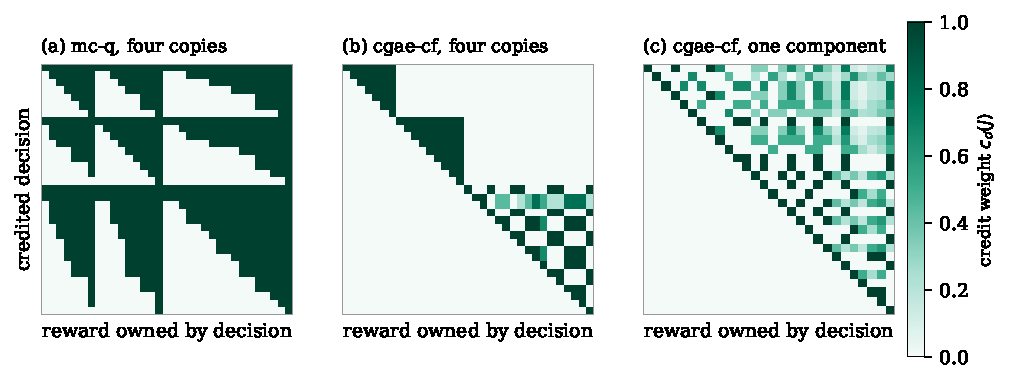
\includegraphics[width=0.82\textwidth]{../figures/fig_credit_matrix.pdf}
\caption{The credit matrix $c_d(j)$, the weight decision $d$ places on the
reward owned by decision $j$, on single episodes. \textbf{(a)} and \textbf{(b)}
are the same episode of the four-copy environment under the same ordering:
return-to-go credits a decision for essentially everything after it, while
causal-order credit is confined to its descendants and is block structured, the
blocks being the three reward-bearing components the estimator found without
being given a partition. \textbf{(c)} is the negative control: one block, so
scoping removes nothing independent.}
\label{fig:credit}
\end{figure}

\subsection{A bias bound for \cflow}
\label{sec:bias}

Proposition~\ref{prop:s} says the unnormalized form is unusable; it does not
say the normalized form is correct. This subsection bounds how far \cflow{}
departs from the closure estimand $A^\star$. The bound is relative: it says how
much bias is added on top of an estimator that is unbiased under (A1).

\begin{assumption}[Bounded score]
\label{as:score}
$\lVert\nabla\log\pi(a\mid s)\rVert \le B$ for all $(s,a)$ visited.
\end{assumption}

\begin{lemma}[Path weights are visit probabilities]
\label{lem:visit}
Under Assumption~\ref{as:time}, $\hat W = [\hat w(d\!\to\!s)]$ is row-stochastic
on non-sink nodes and induces a Markov chain on $\Ascr$ with sinks absorbing.
For this chain, $c_d(e)$ is the probability that the walk started at $d$
visits $e$, so $c_d(e)\in[0,1]$.
\end{lemma}

Define the \emph{re-convergence deficiency} at $d$ in worst-case and
reward-weighted form,
\[
  \delta_d \;=\; \max_{e\in\desc(d)}\bigl(1-c_d(e)\bigr),
  \qquad
  \bar\delta_d \;=\;
  \frac{\sum_{e\in\desc^{*}(d)}\bigl(1-c_d(e)\bigr)\,\rho_{de}\,\lvert\mathrm{owned}[e]\rvert}
       {\sum_{e\in\desc^{*}(d)}\rho_{de}\,\lvert\mathrm{owned}[e]\rvert},
\]
and $\delta=\max_d \delta_d$. Both are computable from a few rollouts without
training.

\begin{proposition}[Bounded bias]
\label{prop:bias}
Under Assumptions~\ref{as:time} and \ref{as:score}, with $\lambda=1$ and
$V\equiv0$:
\begin{enumerate}
\item[(i)] $c_d(e)\in[0,1]$ for every $d$ and every $e\in\desc(d)$;
\item[(ii)] $\bigl\lvert A[d]-A^\star[d]\bigr\rvert
      \;\le\; \bar\delta_d \sum_{e\in\desc^{*}(d)}\lvert\mathrm{owned}[e]\rvert
      \;\le\; \delta_d \sum_{e\in\desc^{*}(d)}\lvert\mathrm{owned}[e]\rvert$;
\item[(iii)] the policy-gradient bias relative to the $A^\star$ estimator obeys
      $\bigl\lVert \nabla J_{\cflow} - \nabla J_{\star}\bigr\rVert
        \le B\,\delta \sum_{e}\lvert\mathrm{owned}[e]\rvert\cdot
                \lvert\anc^{*}(e)\rvert
        \le B\,\delta\,n\,G_{\mathrm{abs}}$,
      with $G_{\mathrm{abs}}=\sum_j\lvert r_j\rvert$;
\item[(iv)] if every node of $\desc^{*}(d)$ has out-degree at most one, then
      $\delta_d=0$ and $A[d]=A^\star[d]$ exactly; more generally $\delta_d=0$
      if and only if $\desc^{*}(d)$ is totally ordered by reachability.
\end{enumerate}
\end{proposition}

The bound is instrumented. Table~\ref{tab:cosine} in \ref{app:cosine} reports
$\bar\delta$ per environment over $100$ untrained rollouts. On multi-site
routing every decision has out-degree one, so $\delta=0$ and \cflow{} coincides
with the closure estimand. Where out-degree exceeds one the deficiency grows
with fan-out: the mean of $1-c_d(e)$ over strict descendant pairs is $0.165$
at four copies, $0.188$ at eight and $0.569$ on the single-component
environment, and the reward-weighted $\bar\delta$ is smaller throughout
($0.079$, $0.073$, $0.408$). Lemma~\ref{lem:visit} is verified directly: $\hat
W$ is row-stochastic to $2.2\times10^{-16}$, $c_d(e)$ never leaves $[0,1]$ over
$21{,}073$ causal edges, and $\sum_e c_d(e)\,\mathrm{owned}[e]$ reproduces the
recursion's output to $1.8\times10^{-15}$. The proposition bounds bias, not
performance: \cdag{} attains $\delta=0$ by construction and performs poorly. It
explains why \cflow{} is safe, not why it is good.

Two remarks complete the analysis. With a critic and $\lambda<1$ the recursion
is exactly GAE in expectation over the causal walk, so the additional bias is
the ordinary bootstrap bias of an imperfect critic. And when owned rewards are
nonnegative, as in every environment here, \cflow's departure from $A^{\star}$
is a per-decision rescaling $A[d]=m_d A^{\star}[d]$ with $m_d\in[0,1]$. A
uniform rescaling cannot change the ascent direction and is removed by the
per-batch advantage standardization, so only the dispersion of $m_d$ can
distort the gradient, through an exact cosine law in its coefficient of
variation. \ref{app:cosine} states, proves and measures this: the credit
direction is preserved to within $8.8\%$ in the worst case and exactly on
multi-site.

%===========================================================================
\section{Experiments}
\label{sec:exp}
%===========================================================================

This section compares \cflow{} against discount-matched PPO and seven
alternative credit rules on six problem configurations. The protocol and the
environments are described first, then the results.

\subsection{Protocol}

All comparisons use common random numbers: every greedy evaluation point, for
every seed and method, scores on one fixed scenario set. Returns are normalized
as $(\text{score}-\text{random})/(\text{heuristic}-\text{random})$, where the
anchors are a random policy and a simple priority rule. We report paired
$t$-tests and Wilcoxon signed-rank tests over $20$ seeds, and count
\emph{collapses} (normalized final $\le0.25$). Every arm uses identical
hyperparameters with no per-arm tuning; \ref{app:repro} gives them together
with the architecture and the evaluation protocol, and \ref{app:defs} defines
every comparator arm.

All results are reported at a $40$-epoch budget. An earlier protocol trained
the scaling benchmark for $15$ epochs, at which the policy has barely moved
(final entropy $0.91$--$0.94$ from $1.00$), and it produced a significant but
spurious result: at two copies \cflow{} measured $0.401$ against \cflowraw's
$0.837$ ($p=0.0043$), which at $40$ epochs becomes $+0.102$ ($p=0.51$), sign
reversed. \ref{app:falsified} documents this convergence-speed effect; the
$15$-epoch cells are retained only as a budget-sensitivity ablation.

\subsection{Environments and their structure}

We use three environment families, all specified in \ref{app:envs}. The first
is a multi-site skills-based routing problem with dedicated per-site
specialists, which is the realistic case. The second is an $N$-copies scaling
benchmark of $N$ structurally independent assignment problems sharing one
policy, in which the independence structure is a controlled parameter; it is
run in a base form, whose anchor is provably optimal, and in a harder form
with headroom above the anchor. The third is a two-stage service line whose
single shared employee pool links every case into one causal component, which
is the negative control. Table~\ref{tab:envs} gives their structural
statistics.

\begin{table}[tbp]
\centering
\caption{Structural statistics, computed from random rollouts before training.
$K$ = reward-bearing causal components; fan-out = mean $|\suc(d)|$;
$S$ = scoping ratio.}
\label{tab:envs}
\begin{tabular}{lccccl}
\toprule
environment & $K$ & top comp.\ share & fan-out & $S$ & character \\
\midrule
multi-site routing & $8.0$ & $15.5\%$ & $\mathbf{1.000}$ & $0.106$ & realistic, most decomposable \\
$N=8$ copies       & $6.3$ & $35.5\%$ & $1.160$ & $0.114$ & scaling endpoint \\
$N=4$ copies       & $3.3$ & $42.4\%$ & $1.137$ & $0.221$ & scaling benchmark \\
$N=4$ copies, hard & $3.1$ & $68.3\%$ & $1.295$ & $0.179$ & scaling benchmark, unsaturated \\
$N=2$ copies       & $2.0$ & $56.1\%$ & $1.020$ & $0.472$ & low-$K$ point \\
single component   & $1.0$ & $100\%$  & $1.387$ & $0.474$ & negative control \\
\bottomrule
\end{tabular}
\end{table}

Two features of Table~\ref{tab:envs} are used repeatedly. $K$ predicts whether
scoping can help, and fan-out predicts whether the successor-combination rule
matters at all. On multi-site the fan-out is exactly $1.000$, so \cflow,
\cgae, \ccap{} and \cflowraw{} are bit-identical there, with identical
learning curves on every seed, which we verify rather than assume.

The structural conditions of Section~\ref{sec:estimand} are checked on $20$
untrained rollouts of each environment. No causal edge points backwards in
time ($0$ violations over $21{,}073$ edges). Every reward firing consumes its
tokens from a single nearest-producer decision ($3{,}157$ of $3{,}157$ rewards
on the four original environments, $915$ of $915$ on the hard variant), and
that decision is $\own(j)$ in every case, as Lemma~\ref{lem:own} requires. The
lemma's consequence was tested directly as well: across $177{,}537$ (decision,
reward) pairs whose owner lies outside the descendant closure, and $48{,}210$
on the hard variant, not one has an ancestry decision inside it. The check is
not vacuous, since rewards have $4.35$ to $10.85$ ancestry decisions on
average, so the configuration Assumption~\ref{as:origin} excludes is available
in these nets and does not arise.

\subsection{Main results}

\begin{figure}[tbp]
\centering
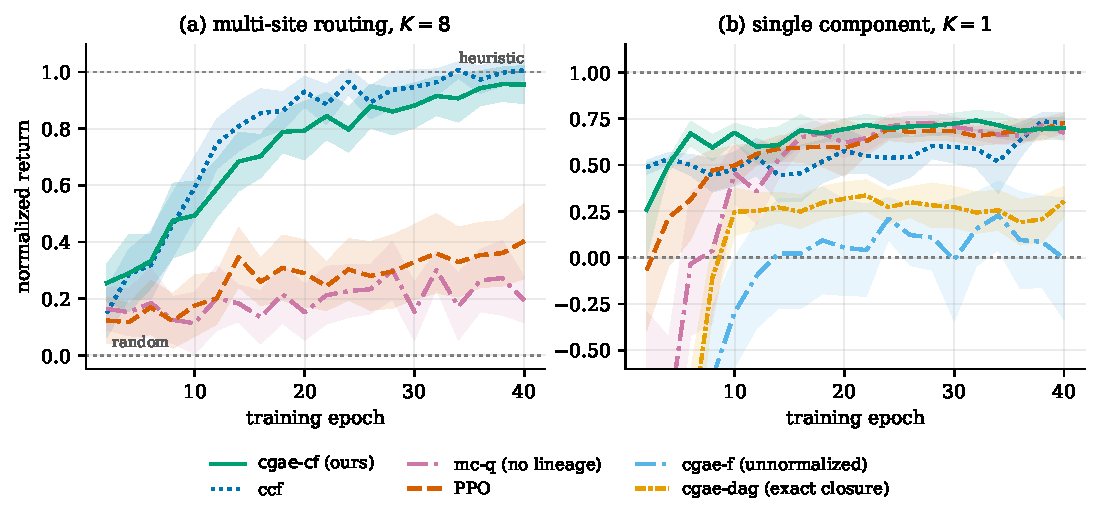
\includegraphics[width=0.86\textwidth]{../figures/fig_curves_v3.pdf}
\caption{Learning curves, mean over $20$ common-random-number seeds with $95\%$
confidence bands; both panels show the same six arms and share the legend.
\textbf{(a)} Where the problem decomposes ($K{=}8$), causal-order credit
separates from PPO by the tenth epoch and reaches the heuristic, while PPO
plateaus below $0.4$ and the lineage ablation \mcq{} stays at or below PPO. On
this environment the fan-out is $1$, so \cflowraw{} is bit-identical to
\cflow{} and its curve lies exactly under it; \cdag{} was not run here.
\textbf{(b)} Where the problem does not decompose ($K{=}1$), \cflow, \ccf,
\mcq{} and PPO are indistinguishable; \cdag{} plateaus at a third of the
attainable return, and \cflowraw{} climbs, turns over and ends near random,
the late deterioration Proposition~\ref{prop:s} anticipates.}
\label{fig:curves}
\end{figure}

\begin{table}[tbp]
\centering
\caption{Normalized final return at $40$ epochs, $20$ common-random-number
seeds per cell, as mean (standard deviation) [collapsed seeds out of $20$].
Dashes are cells not run; bold marks an arm that is significantly best in its
row. On multi-site the causal fan-out is exactly $1$, so \cflow, \cgae, \ccap{}
and \cflowraw{} are the same algorithm and their columns are identical.}
\label{tab:main}
\small
\begin{tabular}{llccccccc}
\toprule
environment & $K$ & \cflow & \cgae & \ccf & \ccap & \cflowraw & \mcq & PPO \\
\midrule
multi-site   & $8.0$ & $0.955$ \tiny{(.15)\,[0]} & $0.955$ \tiny{(.15)\,[0]}
             & $1.005$ \tiny{(.08)\,[0]} & $0.955$ \tiny{(.15)\,[0]} & $0.955$ \tiny{(.15)\,[0]}
             & $0.196$ \tiny{(.18)\,[11]} & $0.403$ \tiny{(.30)\,[6]} \\
$N{=}8$      & $6.3$ & $\mathbf{0.999}$ \tiny{(.03)\,[0]} & ---
             & $0.977$ \tiny{(.06)\,[0]} & --- & $0.741$ \tiny{(.65)\,[3]}
             & --- & $0.804$ \tiny{(.23)\,[0]} \\
$N{=}4$      & $3.3$ & $0.980$ \tiny{(.09)\,[0]} & $\mathbf{0.995}$ \tiny{(.03)\,[0]}
             & $0.974$ \tiny{(.10)\,[0]} & $0.971$ \tiny{(.10)\,[0]} & $0.989$ \tiny{(.03)\,[0]}
             & $0.562$ \tiny{(.29)\,[5]} & $0.715$ \tiny{(.27)\,[1]} \\
$N{=}4$ hard & $3.1$ & $0.405$ \tiny{(.09)\,[1]} & $0.388$ \tiny{(.13)\,[4]}
             & $0.351$ \tiny{(.10)\,[2]} & $0.422$ \tiny{(.12)\,[2]} & $-1.588$ \tiny{(.48)\,[19]}
             & $0.099$ \tiny{(.15)\,[18]} & $0.183$ \tiny{(.13)\,[15]} \\
$N{=}2$      & $2.0$ & $\mathbf{0.882}$ \tiny{(.18)\,[1]} & $0.797$ \tiny{(.30)\,[3]}
             & $0.799$ \tiny{(.30)\,[3]} & $0.761$ \tiny{(.43)\,[3]} & $0.751$ \tiny{(.34)\,[4]}
             & $0.651$ \tiny{(.39)\,[5]} & $0.802$ \tiny{(.30)\,[3]} \\
single comp. & $1.0$ & $0.699$ \tiny{(.14)\,[0]} & $0.643$ \tiny{(.19)\,[1]}
             & $0.727$ \tiny{(.13)\,[0]} & $0.722$ \tiny{(.15)\,[0]} & $-0.006$ \tiny{(.75)\,[10]}
             & $0.675$ \tiny{(.10)\,[0]} & $0.729$ \tiny{(.12)\,[0]} \\
\bottomrule
\end{tabular}
\end{table}

Figure~\ref{fig:curves} shows the learning curves at the two ends of the $K$
range and Table~\ref{tab:main} the final numbers; Table~\ref{tab:paired} in the
appendix gives the paired tests in full. Four observations summarize them.

\paragraph{Against PPO the effect is large where $K$ is large.} On multi-site
\cflow{} improves normalized return by $+0.552$ ($19$W/$1$L, $p<0.0001$) and
collapses on $0$ of $20$ seeds against PPO's $6$. The paired gains are $+0.194$
($p=0.0019$) at eight copies, $+0.264$ ($p=0.0009$) at four and $+0.222$
($p<0.0001$) on the hard four-copy variant, where PPO collapses on $15$ of $20$
seeds. At two copies ($+0.080$, $p=0.34$) and at $K{=}1$ ($-0.030$) the effect
is absent. The effect is therefore present at the four high-$K$ configurations
and absent at the two low-$K$ ones, as Proposition~\ref{prop:k} predicts. The
multi-site collapse is not a tuning artifact: a one-knob grid around the shared
setting (learning rate, GAE $\lambda$, entropy bonus; $20$ seeds each, at
eight episodes per epoch) leaves PPO between $0.15$ and $0.28$ with $9$ to $14$
seeds collapsed in every cell, none better than the shared setting
(\ref{app:repro}).

\paragraph{The gain is located in the causal restriction.} The lineage
ablation \mcq{} is the same SMDP return-to-go with the causal restriction
removed and everything else held fixed. It loses to \cflow{} wherever scoping
is possible, by margins tracking $K$: $+0.760$ on multi-site ($20$W/$0$L),
$+0.418$ at four copies and $+0.306$ on the hard variant (all $p<0.0001$). At
two copies the difference is $+0.230$ with $p=0.010$ on the paired $t$-test but
$0.08$ after Holm correction and $0.11$ on the signed-rank test, so we count it
as suggestive only. Where there is nothing to scope it is null ($+0.024$,
$p=0.52$). On multi-site the ablation even finishes below PPO ($-0.207$,
$p=0.018$).

\paragraph{Against other bounded causal schemes the effect is null.} Versus
\cgae{}, \ccf{}, \ccap{} and \cflowraw{} the paired difference spans $-0.015$
to $+0.009$ at four copies, $-0.040$ to $+0.056$ on the single-component
environment and $+0.080$ to $+0.204$ at two copies, with every $p\ge0.27$
except the $N{=}2$ minimum of $0.052$. On the hard variant the spread against
\cgae, \ccf{} and \ccap{} is $-0.017$ to $+0.054$ with every $p\ge0.11$, and
on multi-site \ccf{} is numerically ahead ($-0.050$, $p=0.21$). An earlier
version of this work, at a shorter budget and fewer seeds, reported a
significant advantage over \ccf{} on multi-site; at the stated protocol the
sign reverses and the difference is null.

\paragraph{On the negative control the method is null, as predicted.} On the
single-component environment \cflow{} is $-0.030$ against PPO ($p=0.46$) and
seven arms lie within $0.06$ of one another: $K=1.0$, one component holds all
the reward mass, and there is nothing to scope. This environment is also where
the ablations separate, as the next subsection shows.

\subsection{The successor normalization is necessary}
\label{sec:normneeded}

\begin{table}[tbp]
\centering
\caption{Single-component environment ($K{=}1$), $20$ seeds, normalized final
return, paired against \cflow. Only two rungs of the ladder are significant.}
\label{tab:ablation}
\begin{tabular}{lccl}
\toprule
variant & final (SD) & collapses & paired vs \cflow \\
\midrule
\cfgae     & $0.739$ {\tiny(0.11)} & $0$ & $-0.040$ ($p=0.27$) \\
PPO        & $0.729$ {\tiny(0.12)} & $0$ & $-0.030$ ($p=0.46$) \\
\ccf       & $0.727$ {\tiny(0.13)} & $0$ & $-0.028$ ($p=0.54$) \\
\ccap      & $0.722$ {\tiny(0.15)} & $0$ & $-0.023$ ($p=0.55$) \\
\cflow     & $0.699$ {\tiny(0.14)} & $0$ & --- \\
\mcq       & $0.675$ {\tiny(0.10)} & $0$ & $+0.024$ ($p=0.52$) \\
\cgae      & $0.643$ {\tiny(0.19)} & $1$ & $+0.056$ ($p=0.36$) \\
\cdag      & $0.304$ {\tiny(0.19)} & $8$ & $\mathbf{+0.395}$ ($\mathbf{p<0.0001}$) \\
\cflowraw  & $-0.006$ {\tiny(0.75)} & $\mathbf{10}$ & $\mathbf{+0.705}$ ($\mathbf{p=0.0006}$) \\
\bottomrule
\end{tabular}
\end{table}

Table~\ref{tab:ablation} reports the ablation ladder on the negative control.
Two rungs are significant: the predecessor-normalized form \cflowraw{} and the
exact-closure form \cdag{} perform substantially worse, while the choice
between flow-weighted, uniform and sub-stochastic handling does not separate
the remaining arms.

\cflowraw{} deteriorates with training, as Proposition~\ref{prop:s}
anticipates. Averaged over the same $20$ seeds it reaches a best-checkpoint
value of $0.443$ and ends at $-0.006$, a within-run drop of $0.449$ against
$0.089$--$0.136$ for every arm that learns. Ten of its seeds end collapsed
while only two are collapsed at their best checkpoint, and one seed's greedy
curve rises, holds for six evaluation points, then falls while policy entropy
stays flat at $0.18$: a low-entropy poor policy rather than a failure to
explore. This is the direction an error term proportional to the critic would
produce, and we report it as consistent with the mechanism rather than as an
isolation of it. The same arm is also unsafe at the highest-$K$
configuration: at eight copies it measures $0.741\pm0.654$ with $3$ collapsed
seeds against \cflow's $0.999\pm0.025$ and none, and the failure is invisible
at five seeds because it appears as occasional failed runs
(Figure~\ref{fig:divergence} in \ref{app:falsified}). The ordering is
unchanged under a best-checkpoint reading.

\subsection{Exactness of the estimand and empirical performance}
\label{sec:exactness}

\cdag{} computes \eqref{eq:star} by construction and is the unbiased member of
the family under (A1). On the single-component environment it ranks
second-worst of the nine arms, and on the hard four-copy variant it ranks last
(Section~\ref{sec:hard}). One structural reason is visible in
Table~\ref{tab:envs}: on a single-component environment the descendant closure
is most of the remaining episode ($S=0.474$), so the exact estimand approaches
the unscoped return and exactness buys no scoping.

The ordering of the four working arms is not accounted for by any mechanism we
tested. Six candidates were probed and all failed, two of them inverted:
per-state ranking fidelity against a common-random-number counterfactual puts
\cdag{} first, and credit signal-to-noise ratio likewise favours the
lower-performing arm. \ref{app:falsified} reports each probe with the
measurement that rejected it. The only variable that separates the learning
from the deteriorating arms without overlap is final policy entropy
($0.27$--$0.56$ against $0.13$--$0.15$), whose causal status is untested. What
the ladder does support is a narrower claim: within this family, exactness of
the estimand is not what distinguishes the arms that learn from the one that
deteriorates, whereas boundedness of the bootstrap coefficient coincides with
that division on the single-component environment. Section~\ref{sec:hard}
shows that boundedness does not predict a second kind of failure.

\subsection{How far is the anchor from optimal?}
\label{sec:optimum}

Normalized return is measured against a myopic heuristic, so a score of $1$
means \emph{as good as that rule}, not \emph{optimal}. On two of the three
families the gap between them can be computed exactly, and we do so.

A single copy of the $N$-copies net and a single site of the multi-site net
are small enough to solve by backward induction: the state is the clock, the
queue counts by type and the remaining service time of each server; service
times are bounded integers and arrivals are one per unit time, so the recursion
is exact. Because the reported configurations share nothing across copies or
sites, the $N$-copy and four-site optima are $N$ and $4$ times the single-unit
optimum. Three clock conventions are not fixed by the environment source; we
enumerate all eight combinations, evaluate the heuristic under each, and keep
the convention reproducing the simulator's own heuristic, which matches it to
$+0.028$ tasks per copy and $+0.059$ per site. Two optima are relevant. The
anchors never postpone, so the \emph{non-idling} optimum says how good the
normalization's unit is. On $N$-copies and the single-component environment
the learned arms may postpone (Table~\ref{tab:hyper}), so their ceiling is the
unrestricted optimum; on multi-site postponement is disabled for learners and
anchors alike, so there the non-idling optimum is the ceiling.

On $N$-copies the heuristic is exactly optimal: matched-first non-idling
attains $11.1245$ expected completions per copy and so does the non-idling
optimum, as the exchange argument for shortest expected processing time on a
single server predicts. Allowing idling adds $0.0326$ per copy, all of it a
horizon artifact recovered by idling from $t\ge17$ only. On the normalized
scale the anchor sits at $1.000$ and the ceiling for the arms is $1.010$. On
multi-site the single-site non-idling optimum is $20.2892$ against the
heuristic's $20.1643$, so the ceiling is $1.029$; idling would raise it to
$1.104$, but no arm may idle there.

Table~\ref{tab:main} can therefore be read as an optimality gap. Against the
ceiling of $1.010$, \cflow{} attains $98.9\%$ of the achievable return at
$N{=}8$, $97.0\%$ at $N{=}4$ and $87.3\%$ at $N{=}2$, against PPO's $79.6\%$,
$70.8\%$ and $79.4\%$; at $N{=}8$ it closes essentially the whole remaining gap
to a computed optimum. Two consequences run the other way. First, a benchmark
whose optimum is attained by most arms cannot discriminate among them: at
$N{=}8$ and $N{=}4$ the causal arms occupy $0.971$--$0.999$, so the nulls
between \cflow{} and the other bounded schemes there are evidence of
saturation, not of equivalence. Second, multi-site is closer to the same
condition than its larger headroom suggests: \cflow's $0.955$ captures
$92.8\%$ of the achievable improvement and \ccf's $1.005$ captures $97.7\%$,
against PPO's $39.2\%$, so the causal arms reach the three-line rule that
anchors the scale and the null between them is again partly a ceiling effect.
Of the six configurations, only the hard four-copy variant leaves every arm
well below its ceiling, which is why we ran it.

\subsection{An unsaturated scaling benchmark}
\label{sec:hard}

The hard variant makes the per-copy problem a genuine assignment rather than
a binary match: each copy has three task types and two heterogeneous
specialists, one fast on each of the first two types (delay $1$), while the
third type matches neither specialist (delay $3$) and a cross-assignment is
slower still (delay $4$), each plus $U\{0,1\}$ (\ref{app:envs}). The copies
remain independent by construction, with $K=3.1$, fan-out $1.295$ and scoping
ratio $0.179$ (Table~\ref{tab:envs}). The matched-first anchor is not optimal
here, so the ceiling exceeds $1$ by a margin we have not computed; what
matters is that no arm approaches it, the best final value being $0.422$. The
protocol is that of the other $N$-copies cells (\ref{app:repro}).

\begin{table}[tbp]
\centering
\caption{Hard four-copy variant ($K{=}3.1$), $20$ common-random-number seeds,
normalized final return as mean (SD) [collapsed seeds], the paired difference
of \cflow{} minus each arm, and each arm's paired difference against PPO with
wins out of $20$.}
\label{tab:hard}
\small
\begin{tabular}{lcclll}
\toprule
arm & final (SD) & collapses & \cflow{} minus arm & arm minus PPO & \\
\midrule
\ccap      & $0.422$ {\tiny(0.12)} & $2$  & $-0.017$ ($p=0.60$) & $+0.239$ ($p<0.0001$) & $18$W \\
\cflow     & $0.405$ {\tiny(0.09)} & $1$  & --- & $+0.222$ ($p<0.0001$) & $17$W \\
\cgae      & $0.388$ {\tiny(0.13)} & $4$  & $+0.017$ ($p=0.50$) & $+0.205$ ($p=0.0002$) & $16$W \\
\ccf       & $0.351$ {\tiny(0.10)} & $2$  & $+0.054$ ($p=0.11$) & $+0.168$ ($p<0.0001$) & $18$W \\
PPO        & $0.183$ {\tiny(0.13)} & $15$ & $+0.222$ ($p<0.0001$) & --- & \\
\mcq       & $0.099$ {\tiny(0.15)} & $18$ & $+0.306$ ($p<0.0001$) & $-0.084$ ($p=0.07$) & $9$W \\
\cfgae     & $-1.361$ {\tiny(0.49)} & $20$ & $+1.766$ ($p<0.0001$) & $-1.544$ ($p<0.0001$) & $1$W \\
\cdag      & $-1.486$ {\tiny(0.28)} & $20$ & $+1.891$ ($p<0.0001$) & $-1.669$ ($p<0.0001$) & $0$W \\
\cflowraw  & $-1.588$ {\tiny(0.48)} & $19$ & $+1.993$ ($p<0.0001$) & $-1.771$ ($p<0.0001$) & $1$W \\
\bottomrule
\end{tabular}
\end{table}

Table~\ref{tab:hard} reports all nine arms. With headroom, the gap to PPO is
large and the intra-family nulls persist. PPO collapses on $15$ of $20$ seeds
and ends at $0.183$, and the four bounded causal schemes beat it by $+0.168$ to
$+0.239$ on $16$ to $18$ of $20$ seeds ($p\le0.0002$). The lineage ablation is
again null against PPO and loses to \cflow{} on all $20$ seeds. Among the four
schemes that learn the spread is $0.071$ and no pairwise difference is
significant (\cflow{} against \ccf{} $+0.054$, $p=0.11$; against \cgae{} and
\ccap{} within $\pm0.017$). With more than half the scale unclaimed, the
bounded variants remain indistinguishable, so their null on the base family is
not attributable to saturation alone.

Three arms never learn, and boundedness does not predict which. \cflowraw,
\cdag{} and \cfgae{} end below random on $19$, $20$ and $19$ seeds. This is not
the late deterioration of Section~\ref{sec:normneeded}: at the first
evaluation, after three epochs, \cdag{} already returns exactly zero on all
$20$ seeds, \cflowraw{} on $11$ and \cfgae{} on $7$, which means the argmax
policy postpones at essentially every decision. A static diagnostic points at
why. Under a random policy and a constant critic, the standardized advantage
each scheme assigns to postpone decisions on this variant is $-1.05$ to $-1.27$
for \cflow, \ccap{} and \cgae, with no postpone decision receiving a positive
advantage, but $+0.46$ for \cflowraw{} and $+0.32$ for \cdag; on the base
variant every scheme gives postpone a negative advantage. The two cgae-family
arms that fail are thus the two whose credit tells the untrained policy that
idling pays. We read this as consistent with the failure rather than as its
cause, since \ccf{} also gives postpone a mildly positive advantage ($+0.21$)
yet learns, and \cfgae{} is not covered by the diagnostic. Two of the three
failing arms have a bounded bootstrap coefficient, so the observation of
Section~\ref{sec:normneeded} holds on the single-component environment and
does not extend to this failure mode.

At $40$ epochs every arm that learns is still rising slowly (final policy
entropy $0.88$--$0.90$), so these are fixed-budget numbers rather than
converged ones. The gap between \cflow{} and PPO lies between $0.20$ and $0.25$
at each of the last six evaluation points, while the ordering within the family
may still move.

\subsection{Scaling}
\label{sec:scaling}

\begin{figure}[tbp]
\centering
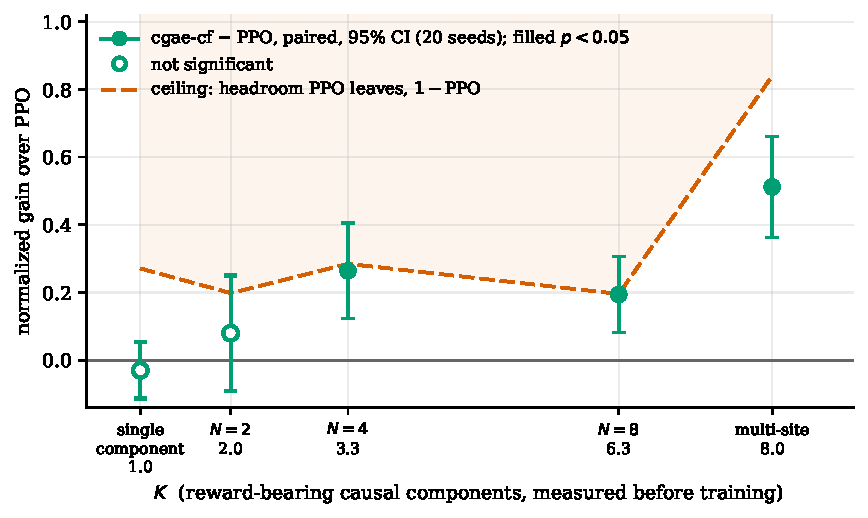
\includegraphics[width=0.68\textwidth]{../figures/fig_k_axis.pdf}
\caption{Paired gain over PPO against $K$, with the headroom PPO itself leaves
drawn per configuration as a ceiling. The gain is absent at $K{=}1$,
significant at the four largest $K$, and positive but not significant at
$K{=}2.0$. At two and eight copies PPO already reaches $0.80$, and the measured
gain sits essentially on the bound ($+0.194$ against a ceiling of $0.196$ at
eight copies); at multi-site PPO leaves $0.597$ unclaimed, of which the method
claims $0.552$. We fit no trend through the six points.}
\label{fig:kaxis}
\end{figure}

The measured gain over PPO is positive at every $K>1$, significant at the four
largest values of $K$, and absent at $K=1$. It is not monotone in $K$, and
Figure~\ref{fig:kaxis} shows why: much of the departure is due to headroom.
At $N{=}8$ every causal arm saturates near the heuristic and PPO reaches
$0.805$, so the headroom above PPO to the ceiling of $1.010$ is $0.206$ and
\cflow{} claims $0.194$ of it; at $N{=}2$ the ceiling is similarly low and the
gain does not reach significance. The hard four-copy variant shows the
converse: at nearly the same $K$ as the base one, PPO leaves $0.817$ unclaimed
and the gain is $+0.222$, so headroom bounds the gain without predicting it.
The defensible claim is therefore that $K$ predicts \emph{whether}
component-scoped credit can help, not \emph{how much}. The $N{=}2$
configuration serves as the low-$K$ end of this curve and for nothing else: at
the converged budget the spread across all seven arms is $0.169$ with nothing
significant.

%===========================================================================
\section{Discussion}
\label{sec:discussion}
%===========================================================================

\subsection{How the empirical gains should be interpreted}
\label{sec:mechanism}

Three things are measured rather than interpreted. Causal-order credit
improves normalized return over discount-matched PPO on the four
configurations with the largest $K$ and is indistinguishable from it on the
two with the smallest. The lineage ablation, which removes only the provenance
restriction, loses to \cflow{} wherever scoping is possible and is null where
it is not, which places the gain in the restriction rather than in the
discounting or the estimator form. And the predecessor-normalized variant
deteriorates late in training on two environments, while every bounded variant
does not; on the hard variant, however, two bounded arms fail from the first
evaluation, so boundedness rules out the late deterioration and not every
failure.

That the gain is caused by variance reduction of the kind
Proposition~\ref{prop:k} describes is a reading of this evidence rather than a
measurement of it. The pattern is consistent with the proposition, but the
proposition assumes conditional independence across components, and the
effect sizes are not a clean function of $K$. At least two channels plausibly
contribute and our design does not separate them. The first is
\emph{decomposition}: restricting a decision's advantage to rewards it could
have influenced removes terms that, under (A1), have zero expected
contribution and nonzero variance. The second is \emph{boundedness}: successor
normalization keeps the credit vector a bounded, low-dispersion object
regardless of the critic, and scoping cuts total credit mass four- to
ninefold, which changes the conditioning of the value-regression target. The
ablation ladder speaks mainly to the second channel. The most defensible
statement is therefore that restricting credit along recorded provenance
produces the gain over PPO, which the ablation establishes, and that among
schemes applying such a restriction, keeping the estimator bounded matters more
than making it exact. Why the bounded variants order as they do is not
settled.

\subsection{A decision rule for practitioners}

Compute $K$ from a handful of random rollouts before adopting anything. If the
problem decomposes, even partially, into weakly coupled sub-streams, such as
parallel lines, multiple sites or segmented resource pools, causal-order credit
offers a cheap drop-in gain with no hand-specified structure. If $K\approx1$,
expect a null; on our negative control the method is neither better nor worse
than the baseline, though one environment is thin evidence for safety in
general. Compute mean fan-out as well: where it is $1$, every variant in
Table~\ref{tab:family} is the same algorithm. Read $K$ alongside a judgement
about resource sharing (Section~\ref{sec:a1scope}), since $K$ sees only the
provenance of executions that happened.

\subsection{Generality beyond Action-Evolution Petri Nets}
\label{sec:generality}

The method is not a modification of RL that applies to an arbitrary
environment. It uses four properties of the formalism: work is carried by
individually identified tokens; every state change is a firing that records
which tokens it consumed and produced, so provenance composes through merges
and splits; rewards are emitted by firings that consume tokens, so each reward
has a well-defined ancestry; and decisions are themselves firings in the same
record. Colored Petri nets \citep{cpn_jensen} satisfy the first three by
definition and need only a marking of which firings are decisions. Entity-flow
discrete-event simulators identify entities individually, so an entity-level
record is obtainable in principle, but the standard trace records an entity's
path through blocks rather than the input--output relation of each event, so
batch, assemble and separate operations are where a token-level record would
have to be added. Process-mining event logs carry a case identifier, which is
coarser than token provenance but enough to recover the same partition where
rewards are earned at case completion and cases do not interact. Models whose
state is aggregate counts do not expose the relation at all. The scope
boundary is the reward structure rather than the domain: the estimator needs
rewards attached to token-consuming firings and enough reward mass in distinct
components for $K$ to exceed one. Admission control and revenue management
satisfy this directly; per-period holding costs would have to be discretized
onto firings first. We have not run a second domain.

\subsection{Limitations}
\label{sec:limitations}

\paragraph{Provenance and decomposability.} The method cannot be applied where
the simulator does not record token identity and firing-level input--output
relations. Instrumenting an existing simulator is usually straightforward but
not free, and its cost outside A-E PN implementations is untested. The gain
requires reward mass in more than one causal component, failing which the
estimator reduces to an unscoped return-to-go. Its value is therefore a
property of the instance rather than of the method.

\paragraph{Near-optimal anchors and near-saturated benchmarks.} On $N$-copies
the anchor is the non-idling optimum and most arms sit within $0.04$ of the
ceiling, so the nulls between \cflow{} and the other bounded rules there say
the benchmark has no resolving power left. The hard variant removes the
ceiling and still does not separate them at $20$ seeds, which is evidence of a
small or absent difference, but its budget is not converged and its optimum is
uncomputed. On multi-site the causal arms reach $0.955$--$1.005$ against a
ceiling of $1.029$, so its clear result is the gap to PPO rather than any
ordering among the causal schemes, and matching a three-line priority rule is
not evidence of operational competitiveness beyond it. The optimum of the
single-component environment is not computed.

\paragraph{Join rewards.} Proposition~\ref{prop:star} needs
Assumption~\ref{as:origin}, and a reward earned by a firing that consumes
tokens last handled by two different decisions violates it. The estimator
still runs, so the failure is silent, which is why we report the condition as
checkable and check it. None of our environments is a merge or assembly
problem; a manufacturing net paying a reward on joining two sub-assemblies is
where it would fail. The condition concerns the reward structure, so it is
independent of (A1) and of $K$.

\paragraph{Assumption~\ref{as:exo} is not verified.} (A1) is argued from A-E
PN semantics plus a modelling judgement about contention, and we know of no
cheap test for it. Where it fails, Propositions~\ref{prop:star} and
\ref{prop:k} lapse; the algebraic results are unaffected but are then relative
to an estimand whose own status has weakened. Our evidence about the coupled
regime rests on a single environment at $K=1$, on which the method is null. We
have not measured intermediate coupling, where (A1) is violated but $K>1$,
which is arguably the most common situation in practice and the one where a
biased scoping rule could do harm. The flexible-worker knob of \ref{app:envs}
is designed to sweep this dial and is not exercised here.

\paragraph{Empirical scope.} All experiments are conducted within the A-E PN
ecosystem: six configurations from three families, one library, one graph
representation, one architecture and one hyperparameter setting. The
configurations share a short horizon, unit completion rewards and a throughput
objective, and two of the three families are synthetic. We can conclude that
provenance-scoped credit helps in decomposable A-E PN task-assignment problems
under this protocol and that the predecessor-normalized form is unsafe in it;
we cannot conclude that the ordering transfers to other encodings, longer
horizons, cost objectives or other discrete-event formalisms. Among the bounded
variants we cannot say which to prefer or why.

\subsection{Three alternative routes on the negative control}
\label{sec:boundary}

Proposition~\ref{prop:k} predicts a null at $K=1$, which raises the question
whether the residual gap on a single-component problem can be closed by giving
the learner more structure by some other route. We tested three, none of which
touches credit assignment: potential-based reward shaping read off the net's
topology, structural input features derived from the conflict graph, and a fix
to the actor architecture. All three are neutral or harmful on the bottleneck
environment. Shaping is policy-invariant \citep{ng1999shaping} yet harmful at
large coefficients, because constant exogenous arrivals make the potential a
noisy value-regression target at a finite budget. Features that are a function
of action type alone are provably redundant, since every action node already
carries its type. The architectural fix repairs a real blindness of the
per-node actor decoder but is neutral here, because the shared pool leaves the
unfixed architecture a marginal path to the same information.
\ref{app:boundary} reports all three. The difficulty of this environment lies
neither in what the learner can observe nor in an avoidable credit bias, and
we state it as an open problem.

\subsection{Future work}

The natural next steps are a coupling sweep that varies shared capacity
continuously and measures performance against (A1) violation directly;
replication in a non-Petri-net discrete-event simulator instrumented to record
entity-level provenance; a cost-minimization problem with mixed-sign,
per-period rewards; and an interventional test of the ablation ordering, an
entropy-bonus manipulation being the most direct.

%===========================================================================
\section{Conclusion}
\label{sec:conclusion}
%===========================================================================

This paper showed that the token provenance an A-E PN simulation records as a
by-product of execution can replace a hand-specified factorization of credit
with a derived one. Running generalized advantage estimation along the
provenance DAG rather than the trajectory index yields a cheap, fork-free
policy gradient that improved on discount-matched PPO by $+0.19$ to $+0.55$ in
normalized return on the configurations whose reward generation is at least
partially decomposable, and was neither better nor worse where it is not. On
the scaling benchmark, where the optimum is computable, the method reaches
$98.9\%$ of it where PPO reaches $79.6\%$. The properties that make this
possible, identified tokens, firing-level input--output records, rewards
emitted by token-consuming firings and decisions that are themselves firings,
are shared by other colored-net and entity-flow simulators, though we have not
tested it outside this one. Two qualifications travel with the result: the
statements about the expected policy gradient hold under a component
mean-exogeneity assumption that segmented capacity makes plausible and shared
capacity does not; and within the estimator family the design choice that
mattered empirically was keeping the bootstrap coefficient bounded rather than
computing the causal estimand exactly, a distinction we can document but have
not explained. A third concerns the benchmarks: on the base scaling family and
on the realistic configuration the causal arms reach a ceiling within a few
percent of the heuristic that anchors the scale, so those benchmarks separate
causal credit from its absence but not the causal schemes from one another,
and only the harder scaling variant leaves room, where they still do not
separate at twenty seeds.


\clearpage
\appendix
\section{Proofs}
\label{app:proofs}
%==========================================================================

The statements are in Section~\ref{sec:theory}; only the arguments are
collected here.

\begin{proof}[Lemma~\ref{lem:own}]
Let $a_j$ be the single nearest producer supplied by
Assumption~\ref{as:origin}. Every token consumed at $j$'s firing descends from
an output token of $a_j$ with no intervening decision, so the backward walk
reaches any other member of $\Ascr(j)$ only by continuing past $a_j$, through
$a_j$'s own consumed tokens. The nearest-producer relation composed
transitively is the successor relation of Section~\ref{sec:method}, so those
decisions are precisely the successor-ancestors of $a_j$:
$\Ascr(j)\subseteq\anc^{*}(a_j)$. By Assumption~\ref{as:time} every successor
edge strictly increases the clock, hence $u_{a_j}\ge u_{d'}$ for every
$d'\in\Ascr(j)$, with equality only at $d'=a_j$; since $\own(j)$ is by
definition the clock-latest member of $\Ascr(j)$, $\own(j)=a_j$.

For the consequence, suppose some $d'\in\Ascr(j)$ lay in $\desc^{*}(d)$. From
$\Ascr(j)\subseteq\anc^{*}(\own(j))$ we have $d'\in\anc^{*}(\own(j))$, i.e.\
$\own(j)\in\desc^{*}(d')$, and $\desc^{*}$ is transitive, so
$\own(j)\in\desc^{*}(d)$ --- contradicting the hypothesis. Hence
$\Ascr(j)\cap\desc^{*}(d)=\emptyset$.
\end{proof}

\begin{proof}[Proposition~\ref{prop:star}]
Write the discarded mass as
$G_d^{\mathrm{full}}-A^{\star}[d]=\Delta_d+\Xi_d$, where $\Delta_d$ collects the
cross-component rewards and
$\Xi_d=\sum \rho_d(t_j)r_j$ runs over the rewards $j$ with $t_j\ge u_d$,
$c(j)=c(d)$ and $\own(j)\notin\desc^{*}(d)$: those in $d$'s own component that
the closure nonetheless omits. It suffices to show each vanishes in the
gradient.

Fix $d$ and condition on $\Fscr_d$. Since $a_d$ is drawn given $\Fscr_d$ and
both quantities are realized afterwards,
\[
  \Ex\bigl[\nabla\log\pi_\theta(a_d\mid s_d)\,X_d \mid \Fscr_d\bigr]
  = \Ex_{a_d}\bigl[\nabla\log\pi_\theta(a_d\mid s_d)\,
    \Ex[X_d\mid\Fscr_d,a_d]\bigr]
\]
for $X_d\in\{\Delta_d,\Xi_d\}$. For $X_d=\Delta_d$ the inner expectation is
free of $a_d$ by Assumption~\ref{as:exo}. For $X_d=\Xi_d$, a reward $j$ in that
sum has $\own(j)\notin\desc^{*}(d)$, so by Lemma~\ref{lem:own}
$\Ascr(j)\cap\desc^{*}(d)=\emptyset$: no decision of $j$'s ancestry is a
descendant of $d$, hence no descendant of $a_d$ lies on $j$'s provenance. Along
the realized execution $r_j$ is therefore not influenced by $a_d$, since $r_j$
is a deterministic function of the tokens consumed at its firing and none of
them descends from $a_d$. Passing from that statement to
$\Ex[\Xi_d\mid\Fscr_d,a_d]=\Ex[\Xi_d\mid\Fscr_d]$ requires the same
mean-exogeneity condition as for $\Delta_d$, now applied to within-component
rewards whose owner falls outside the closure; we assume it in that form, and
Section~\ref{sec:a1scope} discusses the channels that would break it, which are
the same in both cases.

The step through Lemma~\ref{lem:own} is where Assumption~\ref{as:origin} is
consumed, and it cannot be replaced by a time-order argument. Ownership is the
clock-latest decision of $\Ascr(j)$, which on its own does \emph{not} prevent an
\emph{earlier} member of $\Ascr(j)$ from lying in $\desc^{*}(d)$ while the owner
does not: that is exactly the configuration a join reward creates, and there
$r_j$ is a genuine provenance descendant of $a_d$ sitting in $\Xi_d$, where the
argument above would assume it away. Assumption~\ref{as:origin} excludes it.

In both cases the inner expectation is some $\bar X_d$ not depending on $a_d$,
so the outer expectation is
$\bar X_d\,\Ex_{a_d}[\nabla\log\pi_\theta(a_d\mid s_d)\mid\Fscr_d]
 =\bar X_d\,\nabla_\theta\sum_a \pi_\theta(a\mid s_d)=\bar X_d\,\nabla_\theta 1=0$
by the score-function identity. The baseline term contributes zero by the same
identity. Summing over $d$ and taking total expectation gives the claim.
\end{proof}

\begin{proof}[Proposition~\ref{prop:k}]
Conditionally on $s_d$ the baseline is a constant, so it does not affect either
variance. By conditional independence
$\Var(\sum_k R_k\mid s_d)=\sum_k \Var(R_k\mid s_d)=\sum_k\sigma_k^2$, which is
the first equality; the second is immediate. Under
$\sigma_k^2\approx\sigma^2$ the ratio is $K\sigma^2/\sigma^2=K$, and standard
deviation scales as the square root.
\end{proof}

\begin{proof}[Lemma~\ref{lem:visit}]
Row-stochasticity is \eqref{eq:sucsum}. By Assumption~\ref{as:time} the DAG is
acyclic, so a walk visits any node at most once; consequently the events
$\{\text{the walk's initial segment is }\pi\}$, indexed by the distinct paths
$\pi: d\rightsquigarrow e$, are pairwise disjoint and their union is exactly the
event that the walk visits $e$. Each has probability
$\prod_{(x\to y)\in\pi}\hat w(x\!\to\!y)$, and summing gives $c_d(e)$. A
probability lies in $[0,1]$.
\end{proof}

\begin{proof}[Proposition~\ref{prop:bias}]
(i) is Lemma~\ref{lem:visit}. For (ii), telescoping of $\rho$ gives
$A^\star[d]-A[d]=\sum_{e}\bigl(1-c_d(e)\bigr)\rho_{de}\,\mathrm{owned}[e]$;
take absolute values, use $\rho\le1$ and $0\le 1-c_d(e)\le\delta_d$, and note
the middle expression is exactly $\bar\delta_d$ times the total owned mass.
For (iii), the two estimators differ only through the summand, so
$\nabla J_{\cflow}-\nabla J_{\star}
 =\Ex\bigl[\sum_d (A[d]-A^\star[d])\nabla\log\pi_d\bigr]$; apply the triangle
inequality, then (ii) and Assumption~\ref{as:score}, and reindex the double sum
by owner, each $e$ being counted once per ancestor. For (iv), if out-degree is
at most one throughout $\desc^{*}(d)$ the walk is deterministic and visits every
descendant, so $c_d(e)=1$; conversely $c_d(e)=1$ for all $e$ says every maximal
walk from $d$ meets every descendant, which is total order by reachability.
\end{proof}


\section{Estimator definitions and additional remarks}
\label{app:defs}
%===========================================================================

Every arm compared in Section~\ref{sec:exp} differs from every other only in
how the per-decision target $Q[d]$ is formed. All of them are consumed
identically---the policy uses $A_d=Q[d]-V(s_d)$ and the value head regresses on
$Q[d]$---so the comparison isolates the credit rule and nothing else. Throughout,
$u_d$ is decision $d$'s clock, $t_j$ reward $j$'s firing time,
$\rho_d(t)=e^{-\beta\max(0,t-u_d)}$ the SMDP discount, $\Ascr(j)$ the decisions
on $j$'s lineage, $c(\cdot)$ the causal-component map and $\own(\cdot)$,
$\suc(\cdot)$, $\desc^{*}(\cdot)$ as in Sections~\ref{sec:method}
and~\ref{sec:estimand}.

\paragraph{Non-causal reference points.}
\begin{itemize}
\item \textbf{PPO} is the unmodified baseline: ordinary GAE along the trajectory
index with the SMDP discount, $A_t=\delta_t+\gamma\lambda A_{t+1}$.
\item \mcq{} (\emph{the lineage ablation}) is the plain Monte-Carlo SMDP
return-to-go, $Q[d]=\sum_{j:\,t_j\ge u_d}\rho_d(t_j)\,r_j$. Every decision sees
every subsequent reward whether or not it caused it. It shares the estimator
\emph{form} of the causal Monte-Carlo schemes ($\lambda=1$, no bootstrap,
wall-clock discount) and differs from them only by dropping the causal
restriction, which is exactly what makes it the ablation that prices the
lineage. It needs no token DAG.
\end{itemize}

\paragraph{Component-scoped schemes.} These restrict \emph{which} rewards a
decision sees, keeping the Monte-Carlo return-to-go.
\begin{itemize}
\item \lrq{} credits $d$ with the full discounted mass of every reward on whose
lineage it sits, $Q[d]=\sum_{j:\,d\in\Ascr(j)}\rho_d(t_j)r_j$. A reward with $k$
lineage decisions contributes its whole mass to all $k$ of them, so this is a
per-decision hindsight $Q$-sample and \emph{not} a return decomposition; it must
never be summed as a return. It is the scheme single-owner attribution
(Section~\ref{sec:method}) replaces.
\item \ccf{} builds the realized causal-component partition of
Section~\ref{sec:estimand} by union-find over each reward's lineage, then credits
$Q[d]=\sum_{j:\,c(j)=c(d),\,t_j\ge u_d}\rho_d(t_j)r_j$: its own component's
return-to-go. Because the partition is computed from the \emph{realized}
episode, component membership can itself depend on the action taken.
\item \sccf{} replaces that realized partition with a static, topology-only one
derived from the net's structure, which is action-invariant by construction. It
is reported here for completeness; it does not appear in the main tables.
\end{itemize}

\paragraph{Component-filtered GAE.}
\cfgae{} takes \ccf's partition but consumes it through PPO's own recursion
rather than as a Monte-Carlo sample: for each component it runs the ordinary
SMDP-GAE over the step-reward stream masked to that component, and each decision
reads the advantage from its own component's pass. Its $K=1$ limit is therefore
PPO \emph{exactly}---the mask is identically one and the recursion is
term-for-term PPO's---whereas every Monte-Carlo scheme above degenerates at
$K=1$ to \mcq, a different estimator that merely happens to score similarly.
That exactness is why \cfgae{} is the right comparator for "does the
\emph{partition} help, holding the estimator form fixed".

\begin{algorithm}[tbp]
\caption{Causal-order advantage estimation (\cflow)}
\label{alg:cflow}
\begin{algorithmic}[1]
\State \textbf{input:} decisions $\Ascr$ with clocks $u_d$; token history;
       critic values $V[\cdot]$; $\lambda$, $\beta$
\State build $\suc(\cdot)$ and $w(\cdot\!\to\!\cdot)$: one backward
       nearest-producer walk per consumed token
\State $\mathrm{owned}[d]\gets 0$ for all $d$
\ForAll{rewards $r_j$}
  \If{$\Ascr(j)=\emptyset$}
    \State \textbf{continue} \Comment{exogenous: enters no decision's credit}
  \EndIf
  \State $\mathrm{owned}[\own(j)] \mathrel{+}= r_j$
         \Comment{latest decision on $j$'s lineage}
\EndFor
\ForAll{$d\in\Ascr$ in decreasing $u_d$}
  \State $S \gets \suc(d)\setminus\{d\}$
  \If{$S=\emptyset$}
    \State $A[d]\gets \mathrm{owned}[d]-V[d]$ \Comment{causal sink}
  \Else
    \State $R\gets\sum_{s\in S} w(d\!\to\!s)$
    \If{$R>0$}
      \State $\hat w(d\!\to\!s)\gets w(d\!\to\!s)/R$ \textbf{for} $s\in S$
    \Else
      \State $\hat w(d\!\to\!s)\gets 1/|S|$
             \Comment{no attributable inflow: the equal-share case}
    \EndIf
    \State $A[d]\gets \mathrm{owned}[d]-V[d]
            +\sum_{s\in S} \hat w(d\!\to\!s)\,\rho(u_s\!-\!u_d)\,
             \bigl(V[s]+\lambda A[s]\bigr)$
  \EndIf
\EndFor
\State \textbf{return} $Q[d]=A[d]+V[d]$ for all $d$
\end{algorithmic}
\end{algorithm}

\paragraph{The causal-order family.} These run GAE's recursion along the
provenance DAG, differing only in the edge coefficient $c(d\!\to\!s)$ of
\eqref{eq:cflow}; Table~\ref{tab:family} collects the coefficients and the two
sums that matter.
\begin{itemize}
\item \cflow{} (\emph{the method}) uses $\hat w = w/R$, normalized over
successors.
\item \cgae{} uses $1/|\suc(d)|$, the equal-share special case.
\item \cflowraw{} uses the raw flow weight $w$, normalized over predecessors---
the natural formulation, and the one Proposition~\ref{prop:s} shows to be
unbounded.
\item \ccap{} uses $w/\max(R,1)$, which only ever divides, so both the
predecessor and successor sums are at most one. It prices the
share-versus-but-for choice of Remark~\ref{rem:p}.
\item \cdag{} abandons path weighting and uses set semantics: it credits each
decision with each descendant's owned reward exactly once, computing
$A^{\star}$ of \eqref{eq:star} directly. It is the unbiased member of the
family (Proposition~\ref{prop:star}).
\item \textsc{cgae-cf2} is not an ablation of any design choice but a different
DAG construction: \cflow{} with \textsc{postpone} made transparent to the
nearest-producer walk. It appears only in the discussion of that specification
wrinkle.
\end{itemize}

\paragraph{Postponement.} In every causal scheme a \textsc{postpone} decision
receives, in place of a lineage credit, the SMDP
temporal-difference advantage $e^{-\beta\tau}V(s')-V(s)$, so that every arm
gives postponement consistent support.

\begin{remark}[Why single-owner attribution rather than \lrq's lineage sample]
\lrq{} gives each reward's full mass to every decision on its lineage, so
summing its output over decisions overcounts the return by a factor that grows
with lineage depth. Single-owner attribution makes ownership a partition, which
is what turns the estimator into a return decomposition and lets the unrolled
form \eqref{eq:unroll} be read as a weighting of each reward. It also removes a
bias \lrq{} carries in the opposite direction: restricting credit to one
lineage drops the rewards that sibling lineages---the roads not taken at
$d$---would have earned, and those are causal descendants of alternative actions
at $d$, hence not mean-independent of $a_d$.
\end{remark}

\begin{remark}[Shared random streams and Assumption~\ref{as:exo}]
\label{rem:rng}
With a single global random stream, changing $a_d$ can shift the order in which
cross-component events consume random draws, so their \emph{realized} values may
differ across counterfactual actions. This affects the realized $\Delta_d$ but
not $\Ex[\Delta_d\mid\Fscr_d,a_d]$, so Assumption~\ref{as:exo}---which is a
statement about conditional means---is unaffected. The measurements in
Section~\ref{sec:exp} that fork the simulator under common random numbers
exploit exactly this distinction.
\end{remark}

%===========================================================================
\section{The relative bound and the cosine law}
\label{app:cosine}
%==========================================================================

Section~\ref{sec:bias} summarizes this appendix. Proposition~\ref{prop:bias}(iii)
bounds an absolute quantity whose bound scales with $n$, and no bound on the
\emph{ratio} of gradient norms can exist, since near a stationary point the
denominator vanishes while the numerator need not. The useful relative statement
is about \emph{direction}, and for this estimator it is available in closed
form.

\begin{assumption}[Nonnegative owned rewards]
\label{as:pos}
$\mathrm{owned}[e]\ge0$ for all $e$.
\end{assumption}

This holds in every environment we study---throughput and completion rewards
are nonnegative, and we verified that no decision receives negative owned
reward in any measured episode---but it is a property of the reward model, not a
theorem, and estimators for cost-minimization problems with mixed-sign rewards
would need the general form of Proposition~\ref{prop:bias}(ii) instead.

Recall the \emph{reward-weighted deficiency} $\bar\delta_d$ of
Section~\ref{sec:bias}, whose absolute values Assumption~\ref{as:pos} makes
redundant, and define its multiplier
\[
  \bar\delta_d=\frac{\sum_e\bigl(1-c_d(e)\bigr)\rho_{de}\,\mathrm{owned}[e]}
                    {\sum_e \rho_{de}\,\mathrm{owned}[e]},
  \qquad
  m_d = 1-\bar\delta_d \in [0,1],
\]
for every $d$ with $A^{\star}[d]\neq0$.

\begin{proposition}[Exact rescaling and an exact cosine law]
\label{prop:rel}
Under Assumptions~\ref{as:time} and \ref{as:pos}, with $\lambda=1$, $V\equiv0$:
\begin{enumerate}
\item[(i)] \textbf{Exact rescaling.} $A[d]=m_d\,A^{\star}[d]$ for every $d$.
\item[(ii)] \textbf{The level of the shrinkage is free.} If $m_d\equiv m$ is
constant, then $\nabla J_{\cflow}=m\,\nabla J_{\star}$: the ascent direction and
the set of stationary points are \emph{identical}, and the factor $m$ is
absorbed by the step size---and removed outright by the per-batch advantage
standardization used throughout. Only the \emph{dispersion} of $m_d$ can distort
the direction.
\item[(iii)] \textbf{Cosine law.} Let $p_d \propto A^{\star}[d]^2$ and let
$\mathrm{CV}$ be the coefficient of variation of $m$ under $p$. Then
$\cos\angle(A, A^{\star}) = (1+\mathrm{CV}^2)^{-1/2}$ exactly, hence
$1-\cos\angle \le \tfrac{1}{2}\mathrm{CV}^2$.
\item[(iv)] $\mathrm{CV}$ is dimensionless, independent of $n$, and computable
from a handful of untrained rollouts.
\end{enumerate}
\end{proposition}

\begin{proof}[Proposition~\ref{prop:rel}]
(i) By Assumption~\ref{as:pos} the denominator of $\bar\delta_d$ is
$A^{\star}[d]$ and its numerator is $A^{\star}[d]-A[d]$, so
$\bar\delta_d = 1 - A[d]/A^{\star}[d]$, which rearranges to (i). (ii) is
immediate from linearity of $\nabla J$ in the per-decision coefficient. For
(iii), write $u=A^{\star}$ and $A_d=m_d u_d$. Then
$\langle A,u\rangle=\sum_d m_d u_d^2=\Ex_p[m]\lVert u\rVert^2$ and
$\lVert A\rVert^2=\sum_d m_d^2u_d^2=\Ex_p[m^2]\lVert u\rVert^2$, so
\[
  \cos\angle=\frac{\Ex_p[m]}{\sqrt{\Ex_p[m^2]}}
           =\frac{\Ex_p[m]}{\sqrt{\Ex_p[m]^2+\Var_p(m)}}
           =\bigl(1+\mathrm{CV}^2\bigr)^{-1/2},
\]
and $(1+x)^{-1/2}\ge 1-x/2$ gives the bound.
\end{proof}


\paragraph{Measured.} Table~\ref{tab:cosine} reports both sides. The identity
(i) holds to machine precision (maximum absolute deviation $1.8\times10^{-15}$
over all episodes), and the cosine law (iii) is exact to
$2.2\times10^{-16}$---these are verifications of algebra, not fits, and the
last two columns agreeing to five decimals in every row is the whole content of
the check. The practical content is the last column: the direction of the
credit vector is preserved to within $8.8\%$ in the worst case, and
\emph{exactly} on multi-site, where out-degree is one so $\bar\delta\equiv0$.
The $\bar\delta$ column is the $\rho$-weighted deficiency of
Section~\ref{sec:bias}, with the absolute values dropped by
Assumption~\ref{as:pos}; at $\beta=0$, $\rho\equiv1$.

\begin{table}[tbp]
\centering
\caption{Proposition~\ref{prop:rel} measured on $100$ untrained rollouts per
environment ($\lambda=1$, $V\equiv0$, $\beta=0$), pooled over all decisions
with $A^{\star}\neq0$. $\mathrm{CV}$ is the $A^{\star2}$-weighted coefficient
of variation of the multiplier $m_d$. Computed by
\texttt{\_diag\_cosine\_law.py}.}
\label{tab:cosine}
\begin{tabular}{lccccc}
\toprule
environment & $\bar\delta$ (mean) & $\mathrm{CV}$ & $\cos\angle$ measured
            & $(1+\mathrm{CV}^2)^{-1/2}$ & $1-\cos\angle$ \\
\midrule
multi-site   & $0.000$ & $0.000$ & $1.00000$ & $1.00000$ & $0.000$ \\
$N{=}4$      & $0.079$ & $0.370$ & $0.93784$ & $0.93784$ & $0.062$ \\
$N{=}8$      & $0.073$ & $0.438$ & $0.91611$ & $0.91611$ & $0.084$ \\
single comp. & $0.408$ & $0.451$ & $0.91156$ & $0.91156$ & $0.088$ \\
\bottomrule
\end{tabular}
\end{table}

\begin{figure}[tbp]
\centering
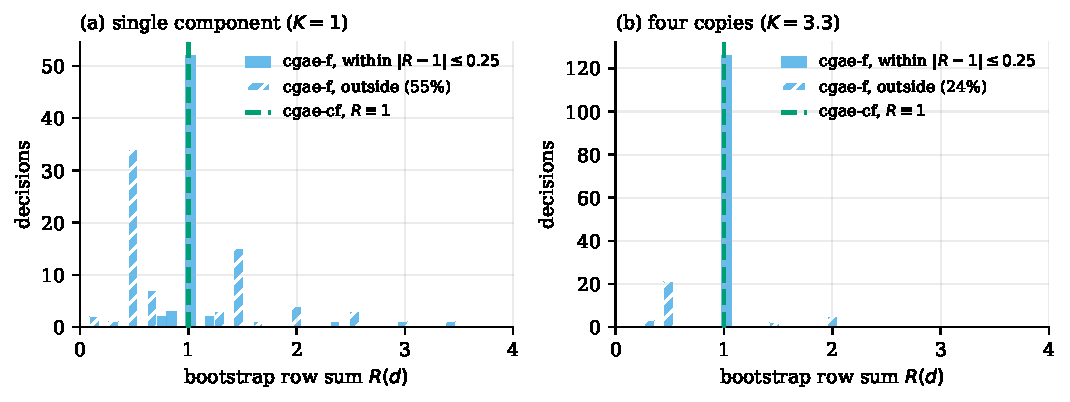
\includegraphics[width=0.80\textwidth]{../figures/fig_rowsum.pdf}
\caption{The bootstrap row sum $R(d)$ over decisions of five random rollouts.
\cflowraw{} leaves it unconstrained---mean $1.008$, standard deviation $0.542$,
range $[0.143,3.429]$ on the single-component environment---so \eqref{eq:defect}
does not vanish; the hatched mass is the $55.3\%$ of decisions ($24.1\%$ at four
copies) where it exceeds a quarter of the critic. \cflow{} divides by $R$, so
its coefficient is the dashed rule at exactly $1$ for every decision. The
aggregate mean of $\approx1$ is what makes the defect easy to overlook: it is a
dispersion problem, not a bias in the mean.}
\label{fig:rowsum}
\end{figure}

\begin{remark}[What the cosine law does and does not cover]
Proposition~\ref{prop:rel}(iii) is a statement about the vectors of
per-decision \emph{coefficients} $A$ and $A^{\star}$, not directly about the
gradients $\sum_d A_d\nabla\log\pi_d$. The two coincide when the score vectors
$\{\nabla\log\pi_d\}$ are orthonormal; in general they differ by a factor
governed by the conditioning of the score Gram matrix, which we do not bound.
We therefore read Table~\ref{tab:cosine} as characterizing the estimator, not
as a guarantee on the realized gradient. As with
Proposition~\ref{prop:bias}, everything is stated \emph{relative} to
$A^{\star}$, whose unbiasedness rests on Assumption~\ref{as:exo}.
\end{remark}
\begin{remark}[The gap between the model and the estimator]
Two idealizations separate Proposition~\ref{prop:k} from what \cflow{} actually
computes. Conditional independence across components is stronger than
Assumption~\ref{as:exo}, which constrains only conditional means: (A1) is what
buys unbiasedness, independence is what buys the variance factor, and an
environment can satisfy the first while only approximately satisfying the
second. And \cflow{} scopes to $\desc^{*}(d)$, which is contained in $c(d)$ and
usually strictly smaller, so it discards more than the model does---which is why
the empirical gain is not a clean function of $K$ (Section~\ref{sec:scaling}).
The proposition should be read as identifying the mechanism and its governing
quantity, not as predicting an effect size.
\end{remark}

\begin{table}[tbp]
\centering
\caption{Paired comparisons against \cflow{} ($20$ seeds, paired $t$-test).
The pattern is uniform on the five base configurations: large and significant
against non-causal or unbounded-coefficient baselines, null against every
bounded causal variant. The hard four-copy variant keeps the first half of
that pattern and breaks the second only for the two bounded arms that never
learn there (Section~\ref{sec:hard}).}
\label{tab:paired}
\small
\begin{tabular}{llrrl}
\toprule
environment & comparator & difference & $p$ & \\
\midrule
multi-site & PPO        & $+0.552$ & $<0.0001$ & $\ast\!\ast\!\ast$ \\
multi-site & \mcq       & $+0.760$ & $<0.0001$ & $\ast\!\ast\!\ast$ \\
multi-site & \ccf       & $-0.050$ & $0.21$    & null \\
$N{=}8$    & PPO        & $+0.194$ & $0.0019$  & $\ast\!\ast$ \\
$N{=}8$    & \cflowraw  & $+0.258$ & $0.0999$  & \\
$N{=}8$    & \ccf       & $+0.021$ & $0.24$    & null \\
$N{=}4$    & \mcq       & $+0.418$ & $<0.0001$ & $\ast\!\ast\!\ast$ \\
$N{=}4$    & \cfgae     & $+0.370$ & $0.0005$  & $\ast\!\ast\!\ast$ \\
$N{=}4$    & PPO        & $+0.264$ & $0.0009$  & $\ast\!\ast\!\ast$ \\
$N{=}4$    & \cgae, \ccf, \ccap, \cflowraw & $-0.015$ to $+0.009$ & $\ge 0.43$ & null \\
$N{=}4$ hard & \cflowraw, \cdag, \cfgae & $+1.77$ to $+1.99$ & $<0.0001$ & $\ast\!\ast\!\ast$ \\
$N{=}4$ hard & \mcq       & $+0.306$ & $<0.0001$ & $\ast\!\ast\!\ast$ \\
$N{=}4$ hard & PPO        & $+0.222$ & $<0.0001$ & $\ast\!\ast\!\ast$ \\
$N{=}4$ hard & \ccf       & $+0.054$ & $0.11$    & null \\
$N{=}4$ hard & \cgae, \ccap & $-0.017$ to $+0.017$ & $\ge 0.50$ & null \\
$N{=}2$    & \mcq       & $+0.230$ & $0.010$   & not after Holm ($0.08$) \\
$N{=}2$    & all other arms & $+0.080$ to $+0.204$ & $\ge 0.052$ & null \\
single comp. & \cflowraw & $\mathbf{+0.705}$ & $\mathbf{0.0006}$ & $\ast\!\ast\!\ast$ \\
single comp. & \cdag     & $\mathbf{+0.395}$ & $\mathbf{<0.0001}$ & $\ast\!\ast\!\ast$ \\
single comp. & PPO, \cgae, \ccap, \cfgae, \ccf, \mcq & $-0.040$ to $+0.056$ & $\ge 0.27$ & null \\
\bottomrule
\end{tabular}
\end{table}

\section{Environments}
\label{app:envs}
%===========================================================================

All three environment families are Action-Evolution Petri Nets built with the
same library and solved by the same agent; they differ in topology, not in
machinery. Each grants reward $1$ per completed task, so return is throughput
over the horizon. Table~\ref{tab:envspec} collects the parameters.

\paragraph{Multi-site skills-based routing (the realistic environment).}
A firm runs four service sites. Each site has its own stochastic arrival stream
of tasks of two types and its own heterogeneous pool of dedicated specialists:
one skilled for each type, fast on their matched type (service delay $1$) and
slow otherwise (delay $3$). A specialist serves a task at its own site and
returns to that site's pool. The decision is which queued task each free worker
takes. Because every worker cycles within its own site, each worker's token
lineage links only decisions that used it, and the episode decomposes into eight
causal components---which is why this environment measures $K=8.0$ and a causal
fan-out of exactly $1$.

The environment also carries a coupling knob we do not exercise in the main
results but which motivates the design: a pool of \emph{flexible} generalists,
usable at any site (delay $2$, type-independent). A flexible worker that serves
site $i$, returns to the shared pool and then serves site $j$ links those sites'
decisions into one component. The local/flexible capacity split therefore traces
the whole independence spectrum---all-dedicated gives $n_{\mathrm{sites}}$
components, all-pooled gives one---instantiating the classical
OR question of resource pooling and flexibility as a single dial over $K$. The
reported configuration is the all-dedicated end.

\paragraph{The $N$-copies scaling benchmark.}
$N$ fully independent single-stage assignment problems in one net, served by one
shared policy, with reward summed over copies. Each copy has its own arrival
stream, queue, busy place and dedicated employee; no place is shared. A copy's
tasks are either \emph{matched} to its employee (service $1+U\{0,1\}$) or
\emph{crossed} (service $3+U\{0,1\}$), so serving matched work first maximizes
throughput. The copies are causally independent by construction, so $K\le N$
with equality whenever every copy emits a reward within the horizon
(Definition~\ref{def:k}). This is the one environment where the independence
structure is a controlled parameter rather than a measured property, which is
what makes it the scaling benchmark; it is deliberately synthetic.

\paragraph{The hard $N$-copies variant.} The same net with a genuine per-copy
assignment. Each copy has two specialists (codes $0$ and $1$) and tasks of
three types, arriving one per unit time with type uniform on $\{0,1,2\}$ and a
warm start of one task of each type. Specialist $k$ serves type $k$ in delay
$1$; type $2$ matches neither specialist and takes $3$; a cross-assignment
(type $0$ to specialist $1$ or the reverse) takes $4$; each plus $U\{0,1\}$.
The decision is therefore which queued task each free specialist takes, and the
matched-first rule that anchors the normalization is not optimal, since it does
not prefer a type-$2$ task to a cross-assignment nor choose between the two
servers. No place is shared across copies, so the independence structure is
unchanged. Section~\ref{sec:hard} reports it at $N=4$; the anchors are
$47.55$ (random) and $75.25$ (heuristic).

\paragraph{The single-component environment (negative control).}
A two-stage service line: cases arrive stochastically, are served at stage one,
then queue for stage two, and reward is emitted on completing stage two. Both
stages draw from \emph{one shared pool of three heterogeneous employees}---two
specialists, fast on their matched type (delay $1$) and slower otherwise
($2$), plus a generalist (delay $3$)---and every employee returns to that same
pool after each service. The shared pool links every case's lineage into a
single causal component, giving $K=1.0$ with one component holding $100\%$ of
reward mass. It is the mechanism's own predicted null, and it is also the
environment of the boundary-condition investigation of
\ref{app:boundary}, where it is called the \emph{bottleneck
environment} because the shared pool is the binding constraint.

\begin{table}[tbp]
\centering
\caption{Environment parameters. Horizon is in simulated time units; the
heuristic is the anchor for the normalization
$(\text{score}-\text{random})/(\text{heuristic}-\text{random})$. The last
column is the exact optimum where we can compute it
(Section~\ref{sec:optimum}), expressed on the normalized scale, so it is the
ceiling any arm in Table~\ref{tab:main} could attain. On $N$-copies the arms
may postpone and the ceiling is the idling-permitted optimum; the anchors never
postpone, and against the non-idling optimum the heuristic is exactly optimal
there ($1.000$). On multi-site neither arms nor anchors may postpone, so the
ceiling is the non-idling optimum. Dashes are configurations whose optimum we
have not computed.}
\label{tab:envspec}
\small
\begin{tabular}{llcccc}
\toprule
environment & structure & horizon & random & heuristic & ceiling \\
\midrule
multi-site routing & $4$ sites $\times$ $2$ dedicated specialists & $20$ & $62.90$ & $80.25$ & $1.029$ \\
$N$-copies, $N=2$  & $2$ independent copies, $1$ employee each & $20$ & $15.87$ & $22.60$ & $1.010$ \\
$N$-copies, $N=4$  & $4$ independent copies, $1$ employee each & $20$ & $31.13$ & $44.60$ & $1.010$ \\
$N$-copies, $N=4$, hard & $4$ independent copies, $3$ types $\times$ $2$ specialists each & $20$ & $47.55$ & $75.25$ & --- \\
$N$-copies, $N=8$  & $8$ independent copies, $1$ employee each & $20$ & $63.20$ & $89.53$ & $1.010$ \\
single component   & $2$ stages, $1$ shared pool of $3$ & $20$ & $9.85$ & $14.78$ & --- \\
\bottomrule
\end{tabular}
\end{table}

\paragraph{Heuristics.} All three anchors are simple priority rules and none
ever postpones. On multi-site, a specialist takes its own matched type first;
failing that a flexible worker is used; failing that any specialist takes
crossed work. On $N$-copies, a binding serving a matched (fast) task is
preferred, otherwise any enabled binding is taken. On the single-component
environment the rule prioritises by stage---work in progress at stage two
before new work at stage one---and within a stage prefers a type-matched
employee. On the hard $N$-copies variant \emph{matched} means the task type
equals the specialist's code, and the rule is otherwise the same. Random baselines sample uniformly from the enabled bindings. Both
anchors are evaluated on the canonical no-postpone variant of each net, so the
normalization scale is a property of the environment rather than of the action
space the learner sees.

%===========================================================================
\section{Training setup and reproducibility}
\label{app:repro}
%===========================================================================

\paragraph{Architecture.} Policy and value networks are separate heterogeneous
graph networks over the assignment-graph representation, each a stack of three
Heterogeneous Graph Transformer convolutions \citep{hu2020hgt} with hidden width
$128$ and two attention heads, with residual connections and dropout. Places and
transitions are distinct node types. The critic pools over node embeddings to
produce a scalar; the actor decodes one logit per enabled action binding from
that binding's node embedding---the asymmetry \ref{app:boundary}
analyses. Input widths are inferred lazily from the first observation, so the
same code runs unchanged across environments with different attribute sets.

\paragraph{Optimization.} All arms share the hyperparameters of
Table~\ref{tab:hyper}; no per-arm tuning was performed, and the causal schemes
inherit the baseline's settings unchanged. This is deliberate---any tuning
advantage would confound the credit comparison---but it also means the reported
numbers are not the best attainable for any arm. For the baseline alone we
checked that this does not explain its multi-site result: a grid of one-knob
departures from the shared setting (policy and value learning rate $10^{-4}$
and $10^{-3}$, $\lambda=0.9$, entropy bonus $0.03$), each on the same $20$
seeds at $40$ epochs of eight episodes, gives final normalized returns of
$0.15$--$0.28$ with $9$--$14$ collapsed seeds per configuration, none better
than the shared setting itself. The grid was run at the smaller per-epoch
budget, so its absolute values sit below the $20$-episode multi-site column of
Table~\ref{tab:main}; it is the ordering within the grid that answers the
tuning question.

\begin{table}[tbp]
\centering
\caption{Hyperparameters, identical for every arm; the two rows that differ by
environment say so.}
\label{tab:hyper}
\small
\begin{tabular}{ll}
\toprule
parameter & value \\
\midrule
algorithm & PPO with clipped surrogate objective \\
epochs & $40$ (converged budget; $15$ and $30$ retained as ablations) \\
episodes per epoch & $20$ (multi-site, single component); $8$ ($N$-copies) \\
minibatch size & $32$ \\
policy / value learning rate & $3\times10^{-4}$ / $3\times10^{-4}$ \\
policy / value update passes & $3$ / $4$ per epoch \\
clip parameter $\varepsilon$ & $0.2$ \\
entropy bonus & $0.01$ \\
KL early-stopping limit & $0.15$ (mean per-state $\mathrm{KL}(\pi_{\mathrm{old}}\Vert\pi)$) \\
discount $\gamma$ / GAE $\lambda$ & $0.99$ / $0.95$ \\
SMDP discount rate $\beta$ & $0.5$ \\
postponement & enabled ($N$-copies, single component); disabled (multi-site) \\
\bottomrule
\end{tabular}
\end{table}

\paragraph{Evaluation protocol.} Every second epoch (every third on
$N$-copies) the greedy (argmax) policy is evaluated on $20$ episodes; the reported \emph{final} value is the last such
point and \emph{best} the maximum over them. All evaluation uses common random
numbers: with the evaluation seed fixed, evaluation episode $i$ always runs
scenario $\mathrm{seed}+i$, so every method, seed and epoch is scored on one
fixed scenario set and arms differ only by policy. This matters more than it
may appear: without it, the measured noise floor on the single-component
environment is $\pm0.231$ standard deviations per evaluation point and
$\pm0.327$ on a paired difference, and drift is inflated by roughly $0.40$ even
for a policy that is not changing. Baselines average $40$ episodes. Seeds
$0$--$19$ are used for every cell, and comparisons are paired seed-by-seed;
we report paired $t$-tests and Wilcoxon signed-rank tests, and where they
disagree we say so.

\paragraph{Determinism.} A single entry point seeds Python's \texttt{random},
NumPy and PyTorch, and is applied to environment construction, network
initialization, rollout collection and evaluation, so a cell is reproducible
from its (environment, method, seed) triple. Paired arms share their network
initialization. Each cell is written to its own result file and runs are
resumable: re-running a sweep trains only the missing cells, which is how the
arm coverage in Table~\ref{tab:main} was filled incrementally.

\paragraph{Cost.} Credit computation is a single backward pass over the
decisions of one episode, $O(|E|)$ in the provenance DAG, measured at
approximately one millisecond per episode. Against a training cell at four
copies this is under $8\%$ of wall-clock time (PPO $7.44$ minutes against
$8.05$); the graph network dominates, and profiling attributes roughly $83\%$
of a cell to the optimizer's repeated forward and backward passes over the
collected graphs. No arm requires forked simulation.

\section{Falsified mechanisms}
\label{app:falsified}

Section~\ref{sec:exactness} reports that the arm computing the causal estimand
exactly is not the best performer, and offers only a partial structural account
of why the remaining variants order as they do. Rather than advance a mechanism
we cannot support, we record every candidate we tested and rejected, with the
measurement that rejected it, so that a reader can judge how much of the
ordering is explained and how much is not. All six were pre-registered in the sense that the
prediction was written into the diagnostic script before it was run.

\subsection{Summary}

\begin{table}[h]
\centering
\caption{Candidate mechanisms for the ablation ordering, and the measurements
that falsified them. ``Inverted'' means the measured quantity ordered the
variants \emph{opposite} to performance.}
\label{tab:falsified}
\small
\begin{tabular}{p{4.1cm}p{5.4cm}l}
\toprule
hypothesis & measurement & outcome \\
\midrule
Postpone is the dominant source of the action-dependence of $R$ &
making postpone transparent leaves $R$ identical across actions on $50.0\%$ of
fork points, down from $68.8\%$; spread on the single-component environment
rises $0.580\to0.947$ &
\textbf{worse} \\[2pt]
Credit decays along chains as $\prod w$, so \cflowraw{} propagates less &
backward propagation mass at causal depth $5$: $0.89$ (\cflowraw) vs $0.95$
(\cflow) &
too small \\[2pt]
Larger credit magnitude gives a larger effective step &
$\mathrm{mean}|Q|$ at two copies: $2.23$ vs $2.22$; $\mathrm{SD}$ $1.10$ vs
$1.12$ &
identical \\[2pt]
Per-state ranking fidelity against a measured counterfactual &
Spearman $\rho$ / top-$1$ agreement with common-random-number counterfactual
return: \cdag{} $+0.681$ / $83.3\%$, \cflow{} $+0.435$ / $33.3\%$ &
\textbf{inverted} \\[2pt]
Credit signal-to-noise ratio (bias--variance) &
between-action signal over within-action noise: \cdag{} $0.959$ (highest),
\cflow{} $0.895$; full range $0.80$--$0.96$ &
\textbf{inverted} \\[2pt]
\cdag's arbitrary $\lambda^{k_{\min}}$ depth weighting &
replacing it with the depth-conditioned weight $\Ex[\lambda^{L}\mid\text{visit}]$
moves correlation with \cflow{} from $0.740$ to $0.748$ &
$\Delta=0.008$ \\
\bottomrule
\end{tabular}
\end{table}

\subsection{Detail}

\paragraph{Postpone transparency.}
Under token-flow postponement a \textsc{postpone} firing re-emits the entire
marking, so it terminates the nearest-producer walk without having caused the
flow, and it carries $2.25$--$2.66\times$ the row sum of production actions. We
therefore expected removing it to make $R$ closer to action-measurable. It does
the opposite. Transparency \emph{redirects} postpone's edges to the true
producers---$0$ production-to-production edges lost, $50$ gained at four copies
and $97$ on the single-component environment---and the recovered edges are
precisely the action-dependent ones. Postpone had been making $R$ look invariant
by discarding information. The resulting variant is also the worst arm we
measured ($0.106$ normalized), so on this environment the more
provenance-faithful graph is the weaker learner---a second instance of the
pattern in Section~\ref{sec:exp}.

\paragraph{Chain decay and credit magnitude.}
Both were attempts to explain a large performance gap by a mechanical property
of the credit vector, and both fail on magnitude grounds: the measured
differences are one to five percent where the performance difference to be
explained was $0.44$ in normalized return.

\paragraph{Ranking fidelity.}
This is the sharpest negative result, because it tests the estimator against
ground truth rather than against another estimator. At a decision state we fork
the simulator once per action under common random numbers and record the
realized discounted return-to-go; differences across branches are then the
causal effect of the action with the exogenous component cancelled. A credit
scheme should rank actions the way that quantity does. On the single-component
environment \cdag{} ranks them \emph{better} than \cflow{} on both measures
while learning far worse. Ranking fidelity at a fixed state therefore does not
determine learning outcome. Caveats: $12$ usable fork points, and the
continuation policy is random, so this measures counterfactual value under
random continuation rather than under the converged policy.

\paragraph{Signal-to-noise.}
We forked each production action under $M$ shared exogenous seeds and formed the
ratio of between-action to within-action credit dispersion---an $F$-ratio for
the quantity a policy gradient integrates. The prediction was that \cdag{},
whose closure sum approaches the unscoped return on a single-component problem,
would show the lowest ratio. It shows the highest. The mechanism was half right
and immaterial: \cdag{} does carry about twice the noise ($0.459$ vs $0.272$),
but it also carries about twice the signal ($0.420$ vs $0.237$), and the
scaling cancels.

\paragraph{The depth-weighting choice.}
\cdag{} weights a descendant's owned reward by $\lambda^{k}$ at minimum causal
depth $k$, which is discretionary: a re-convergent descendant reachable at
depths $2$ and $7$ receives $\lambda^{2}$. We built the principled alternative,
weighting by $\Ex[\lambda^{L}\mid\text{the walk visits } j]$, which coincides
with the closure estimand at $\lambda=1$ and inherits \cflow's depth
distribution conditioned on arrival. It changes almost nothing. The reason is
structural and is worth stating as a positive by-product: since
\[
  c^{\cflow}_d(j)\;=\;\underbrace{\Pr[\text{visit } j]}_{\text{the fan-out gap}}
  \cdot\underbrace{\Ex\bigl[\lambda^{L}\mid\text{visit } j\bigr]}_{\text{depth weighting}},
\]
the two factors are separable, and the closure variants differ from \cflow{}
only by discarding the first. The behavioural difference is the gap itself, not
any detail of how depth is discounted within the closure.

\begin{figure}[tbp]
\centering
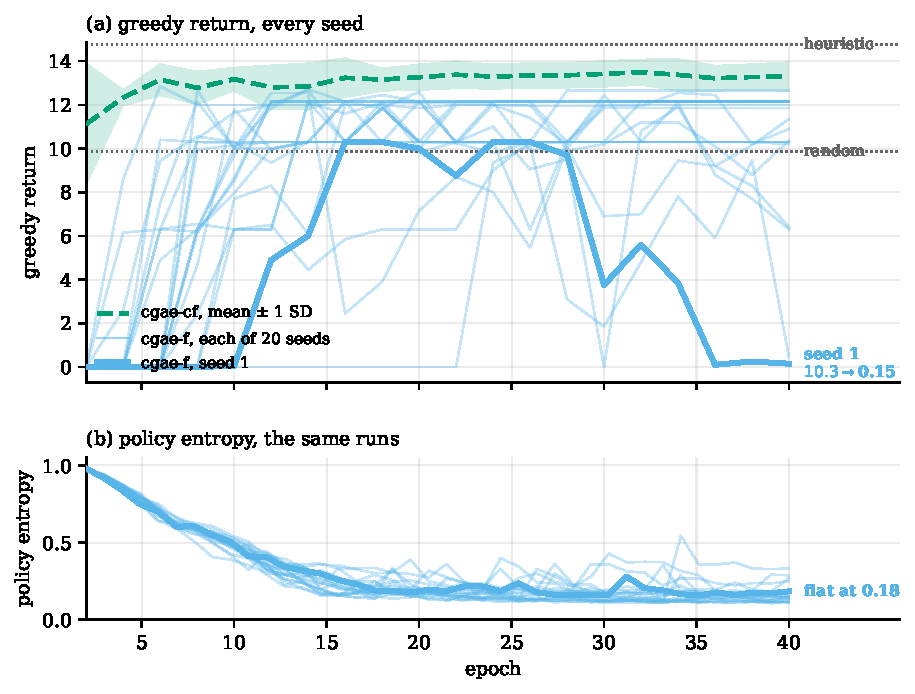
\includegraphics[width=0.88\textwidth]{../figures/fig_divergence.pdf}
\caption{Per-seed behaviour of \cflowraw{} on the single-component environment.
\textbf{(a)} Every \cflowraw{} seed (thin) against \cflow's mean and spread
(dashed, band); $10$ of $20$ \cflowraw{} seeds end collapsed. The emphasised run
is seed $1$: it climbs to $10.3$, holds there for roughly six evaluation points,
then falls to $0.15$---below the random anchor. \textbf{(b)} Entropy over the
same runs, on a shared epoch axis. Seed $1$'s entropy is flat at $0.18$
throughout the collapse, so the end state is a low-entropy poor policy rather
than a failure to explore, which is the pattern Proposition~\ref{prop:s} leads
one to expect when the error term grows with the critic. A mean with a
confidence band does not show this, which is why the behaviour was not apparent
in five-seed comparisons.}
\label{fig:divergence}
\end{figure}

\subsection{Best-checkpoint reading of the ablation ladder}

Table~\ref{tab:ablation} reports final greedy return. Under best-checkpoint
restoration the two significant results and the whole ordering are unchanged:
\cflowraw{} reads $0.443$ {\tiny(0.14)} ($+0.390$ against \cflow, $20$W/$0$L,
$p<0.0001$) and \cdag{} $0.516$ {\tiny(0.15)} ($+0.316$, $19$W/$0$L,
$p<0.0001$), against \cflow's $0.833$ {\tiny(0.08)}, with every remaining arm
within $0.041$ of \cflow{} and no $p$ below $0.13$. The magnitudes shrink
because checkpoint restoration is a partial guard against the late-training
deterioration of Section~\ref{sec:normneeded}.

\subsection{A budget artifact, recorded for the same reason}

At the $15$-epoch budget with $20$ seeds, \cflow{} measured $0.401$ against
\cflowraw's $0.837$ at two copies ($4$W/$14$L, $p=0.0043$)---an apparently
significant deficiency in the method we ship. It is an artifact of
non-convergence. At $40$ epochs the comparison is $+0.102$ ($p=0.51$), sign
reversed. Three measurements identify the cause: a $\lambda$ sweep recovers most
of the deficit ($0.401\to0.579\to0.639$ as $\lambda$ falls
$0.95\to0.85\to0.70$ toward \cflowraw's effective $0.95\times0.896\approx0.851$),
so it is a convergence-\emph{speed} effect; the credit vectors differ by about
one percent; and the outcomes are bimodal with nothing in between. We report
this because it is the clearest evidence in this work that a significant result
at a short budget can be entirely spurious, and it is why
Section~\ref{sec:exp} reports the converged budget throughout.

\subsection{The one surviving correlate}

Across all arms and environments the single variable that separates working from
failing configurations without overlap is \emph{final policy entropy}:
$0.27$--$0.56$ for the four arms that learn, $0.13$--$0.15$ for the three that
fail. Whether this is cause or symptom is untested---a policy in a poor local
optimum will show low entropy regardless of how it arrived---and the decisive
experiment, an entropy-bonus intervention on the failing arms, has not been run.
We state the correlation and its status rather than promoting it to a mechanism.

\subsection{Methodological note}

All six diagnostics share a design feature that may explain their uniform
failure: each measures a \emph{static} property of the estimator under a
\emph{random} policy with random continuations. Training involves a learned
policy that becomes progressively deterministic, and the failures we are trying
to explain unfold over tens of epochs. It is entirely possible that no static,
random-policy property of a credit estimator predicts its training outcome. If
so, that is itself a finding about how credit-assignment methods should be
evaluated, and it argues for interventional rather than observational
diagnostics---consistent with the boundary-condition results of
\ref{app:boundary}, where only active-intervention mechanisms ever moved
the single-component floor.

%===========================================================================
\begin{figure}[tbp]
\centering
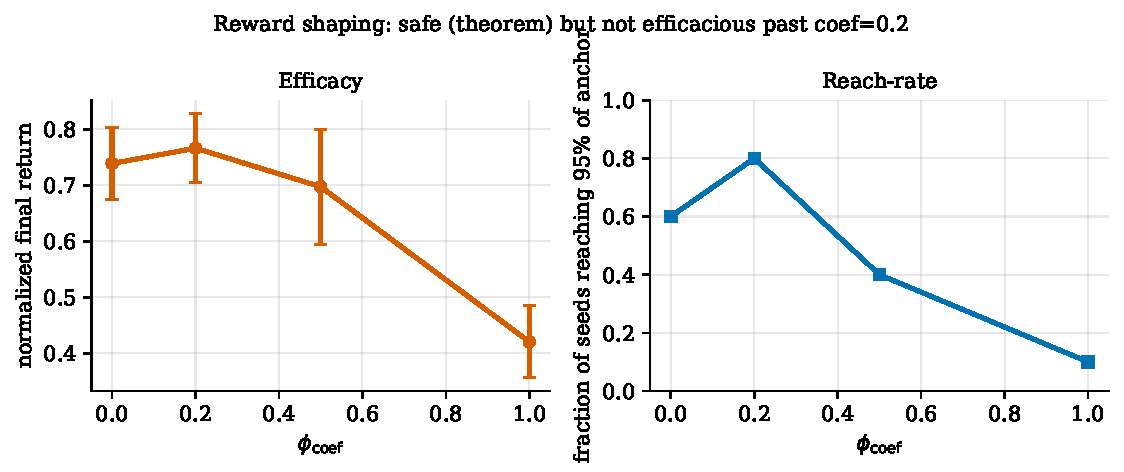
\includegraphics[width=\linewidth]{../figures/fig5_phi_dial.pdf}
\caption{The reward-shaping coefficient dial on the bottleneck environment:
efficacy (left) degrades once past $\phi_{\mathrm{coef}}=0.2$, and the
fraction of seeds reaching $95\%$ of the heuristic anchor (right) degrades
monotonically---safety (Section~\ref{sec:related}, \citealp{ng1999shaping})
and efficacy are independent properties, and this mechanism has the first
without the second at practical training budgets.}
\label{fig:phidial}
\end{figure}

\section{The boundary-condition investigation}
\label{app:boundary}
%===========================================================================

Proposition~\ref{prop:k} predicts that \cflow's variance reduction collapses to
exactly PPO when $K=1$. That is the proposition's own null, and it raises the
question Section~\ref{sec:boundary} summarizes: whether the residual gap on a
genuinely single-component problem can be closed by some other provenance- or
structure-based route. We tested three independent candidates, none of which
touches credit assignment; all three change only what the learner observes. Each
is provably inert or empirically neutral, and two of the three results follow
from a proof rather than from a correlation, which is why we report them rather
than omit them: together they indicate where the difficulty on this environment
does not lie. The environment is the two-stage service line with one shared,
skill-heterogeneous employee pool, called \emph{single component} in
Section~\ref{sec:exp} and the \emph{bottleneck environment} here.
Table~\ref{tab:boundary} summarizes the three outcomes.

\begin{table}[tbp]
\centering
\caption{The boundary-condition investigation, bottleneck environment
($K{=}1$).}
\label{tab:boundary}
\begin{tabular}{lll}
\toprule
mechanism & theoretical status & result \\
\midrule
Reward shaping & policy-invariant, any potential & neutral (0.2) to harmful (1.0), $0$W/$10$L \\
Structural input features & mechanically correct & neutral, $p=.58\to.69$; provably redundant \\
Actor global context & proven to close a real gap & neutral, $p=.91$; gap was already marginal here \\
\bottomrule
\end{tabular}
\end{table}

\paragraph{Protocol, and why it differs.} The three experiments of
\ref{app:boundary} predate the converged-budget re-runs and use the
stochastic suite's standard budget: the single-component environment at $30$
epochs $\times$ $20$ episodes, $10$ seeds, paired seed-by-seed against a
\texttt{ppo\_clip} baseline, reporting normalized final return. That baseline
therefore reads $0.739\pm0.10$ here against $0.729\pm0.12$ in
Table~\ref{tab:ablation}, which is the same arm at $40$ epochs and $20$ seeds;
the difference is budget and seed count, not environment. We did not re-run them
at the longer budget because all three outcomes are nulls or negatives, and a
longer budget cannot convert a null into the positive result that would change
the section's conclusion. The environment is the one described in
\ref{app:envs}; we call it the
\emph{bottleneck environment} to name the mechanism under test rather than the
statistic $K$.

\paragraph{Potential-based shaping.} The shaping term is the SMDP
generalization $F(s,a,s')=e^{-\beta\tau}\Phi(s')-\Phi(s)$, added to every step's
reward, with the potential read off the net's topology:
$\Phi(s)=\sum_p \mathrm{decay}^{\mathrm{hop}(p)}\cdot\min(|p|,\mathrm{cap})$,
a distance-decayed structural backlog in which each place's token count is
weighted by its hop-distance to the nearest reward-emitting transition and
optionally capped. Policy invariance \citep{ng1999shaping} was verified in code
by an exact terminal-value cancellation test rather than merely cited. The
coefficient dial, shown in Figure~\ref{fig:phidial}, reuses one cached
baseline across all four points, so the comparison is paired by construction.

The failure mechanism is worth stating because it is not a property of the
potential's shape. This environment has constant exogenous arrivals---one case
per time unit---so the backlog potential rises as often as it falls, and the
per-step shaping signal is of the same order of magnitude as the entire episode
return. Aggregated over an episode the term telescopes to a constant, exactly as
the theorem promises, but at any finite budget it is a substantially noisier
value-regression target. Safety and efficacy are independent properties, and
this mechanism has the first without the second.

\paragraph{Structural input features.} Two feature sets were appended to each
action node's own inputs: first, whether an action type structurally competes
for a token and with how many rivals, derived from the conflict graph; then,
after that returned a null, the minimum topological hop-distance from an
action's required inputs to the nearest reward-emitting transition. The second
does discriminate between the environment's two action types ($0.656$ against
$0.810$), so the null is not a degenerate-feature artifact.

The redundancy argument is the stronger result and does not depend on either
feature's design. Every action node already carries a one-hot action-type
identity at zero hops. Any scalar that is a function of action type alone is
therefore a deterministic function of information a single learned weight on
that one-hot could reconstruct, so it cannot add representational capacity. This
holds for this architecture on any topology, which is why we report it as a
proof rather than as two failed experiments. A structural feature can only help
if it varies \emph{within} an action type---across markings---which
conflict-degree on a two-node conflict pair provably does not.

\paragraph{Actor architecture.} The blind spot is a property of the
computational graph, not of training. The actor decodes each action's logit from
that action node's own final message-passing embedding; the graph's edges run
strictly along token flow, with no reverse edges at any real observation call
site; so an action's logit can depend on state only through a forward path
reaching it within the network's depth. The demonstration uses a purpose-built
topology of two structurally independent two-stage pipelines: perturbing one
pipeline's downstream marking leaves the other pipeline's action logit
bit-for-bit unchanged ($\Delta=0.000$) under a randomly initialized, untrained
network. Reachability does not depend on learned weights, so no training budget
can close it.

The fix concatenates onto each action node, before decoding, the same pooled
context the critic already computes---an intervention on the actor alone,
leaving the critic and the credit path untouched. On the proof topology it
closes the gap exactly ($\Delta=0.000\to0.528$). On the single-component
environment it is neutral ($0.746\pm0.14$ against $0.739\pm0.10$, $p=.91$), and
the two results are not in tension: that environment's shared resource pool
recycles workers, which gives the unfixed architecture a marginal, accidental
path to the same information within three hops. The blind spot was never total
there, and whatever fraction the fix newly exposes is not decision-relevant
enough to move a well-tuned baseline at this budget. The architectural finding
stands on the proof; the training result bounds its practical value on this
environment only.

\bibliographystyle{elsarticle-harv}
\bibliography{refs}

\end{document}
